% Options for packages loaded elsewhere
\PassOptionsToPackage{unicode}{hyperref}
\PassOptionsToPackage{hyphens}{url}
%
\documentclass[
]{book}
\usepackage{amsmath,amssymb}
\usepackage{lmodern}
\usepackage{iftex}
\ifPDFTeX
  \usepackage[T1]{fontenc}
  \usepackage[utf8]{inputenc}
  \usepackage{textcomp} % provide euro and other symbols
\else % if luatex or xetex
  \usepackage{unicode-math}
  \defaultfontfeatures{Scale=MatchLowercase}
  \defaultfontfeatures[\rmfamily]{Ligatures=TeX,Scale=1}
\fi
% Use upquote if available, for straight quotes in verbatim environments
\IfFileExists{upquote.sty}{\usepackage{upquote}}{}
\IfFileExists{microtype.sty}{% use microtype if available
  \usepackage[]{microtype}
  \UseMicrotypeSet[protrusion]{basicmath} % disable protrusion for tt fonts
}{}
\makeatletter
\@ifundefined{KOMAClassName}{% if non-KOMA class
  \IfFileExists{parskip.sty}{%
    \usepackage{parskip}
  }{% else
    \setlength{\parindent}{0pt}
    \setlength{\parskip}{6pt plus 2pt minus 1pt}}
}{% if KOMA class
  \KOMAoptions{parskip=half}}
\makeatother
\usepackage{xcolor}
\IfFileExists{xurl.sty}{\usepackage{xurl}}{} % add URL line breaks if available
\IfFileExists{bookmark.sty}{\usepackage{bookmark}}{\usepackage{hyperref}}
\hypersetup{
  pdftitle={HW3: Group Project GitHub + Bookdown Setup},
  pdfauthor={Coded in COBOL},
  hidelinks,
  pdfcreator={LaTeX via pandoc}}
\urlstyle{same} % disable monospaced font for URLs
\usepackage{longtable,booktabs,array}
\usepackage{calc} % for calculating minipage widths
% Correct order of tables after \paragraph or \subparagraph
\usepackage{etoolbox}
\makeatletter
\patchcmd\longtable{\par}{\if@noskipsec\mbox{}\fi\par}{}{}
\makeatother
% Allow footnotes in longtable head/foot
\IfFileExists{footnotehyper.sty}{\usepackage{footnotehyper}}{\usepackage{footnote}}
\makesavenoteenv{longtable}
\usepackage{graphicx}
\makeatletter
\def\maxwidth{\ifdim\Gin@nat@width>\linewidth\linewidth\else\Gin@nat@width\fi}
\def\maxheight{\ifdim\Gin@nat@height>\textheight\textheight\else\Gin@nat@height\fi}
\makeatother
% Scale images if necessary, so that they will not overflow the page
% margins by default, and it is still possible to overwrite the defaults
% using explicit options in \includegraphics[width, height, ...]{}
\setkeys{Gin}{width=\maxwidth,height=\maxheight,keepaspectratio}
% Set default figure placement to htbp
\makeatletter
\def\fps@figure{htbp}
\makeatother
\setlength{\emergencystretch}{3em} % prevent overfull lines
\providecommand{\tightlist}{%
  \setlength{\itemsep}{0pt}\setlength{\parskip}{0pt}}
\setcounter{secnumdepth}{5}
\usepackage{booktabs}
\ifLuaTeX
  \usepackage{selnolig}  % disable illegal ligatures
\fi
\usepackage[]{natbib}
\bibliographystyle{plainnat}

\title{HW3: Group Project GitHub + Bookdown Setup}
\author{Coded in COBOL}
\date{2022-08-03}

\begin{document}
\maketitle

{
\setcounter{tocdepth}{1}
\tableofcontents
}
\hypertarget{table-of-contents}{%
\chapter{Table of Contents}\label{table-of-contents}}

\textbf{2. Introduction}

\textbf{3. About Us}

\begin{itemize}
\tightlist
\item
  3.1 Yuchen
\item
  3.2 Nikita
\item
  3.3 Ben
\item
  3.4 Peiyue
\item
  3.5 Winnifer
\item
  3.6 Jalal
\end{itemize}

\textbf{4. Housing}

\begin{itemize}
\tightlist
\item
  4.1 How to Find a Sublease
\item
  4.2 Sublease Mastersheet
\item
  4.3 Dorm Options
\item
  4.4 Luxury Apartments
\end{itemize}

\hypertarget{introduction}{%
\chapter{Introduction}\label{introduction}}

We are Coded in Cobol. Our proposal is to create a detailed e-guide for newly admitted MBAn students. This guide can help students get familiar with the campus environment and make full use of the resources around them effectively.

In class yesterday we talked with you about the fact that multiple groups are pursuing a similar idea. We plan to meet with these groups after submitting the proposal to split the tasks into three parts and then combine our three websites into one big website. Some specifics on the things we want to cover are:

\hypertarget{what-we-plan-to-cover}{%
\section{What We Plan to Cover}\label{what-we-plan-to-cover}}

\begin{itemize}
\tightlist
\item
  Dining plan/meal prep tips
\item
  Best local restaurants and bars
\item
  Fun things to do
\item
  Technology tips
\item
  Most Instagrammable Spots In Michigan
\item
  Transportation Tips
\item
  Study Spots
\item
  Sports
\end{itemize}

\hypertarget{about-us}{%
\chapter{About Us}\label{about-us}}

In this section you can get to know more about the members of Coded in COBOL.

\hypertarget{yuchen-gao}{%
\section{Yuchen Gao}\label{yuchen-gao}}

Hello! My name is Yuchen Gao. I'm currently a master student pursuing a \href{https://michiganross.umich.edu/graduate/master-of-business-analytics}{MBAn} degree from the Ross School of Business at the University of Michigan. I have an undergraduate degree in Information Science from the \href{https://www.si.umich.edu/}{School of Information} at the University of Michigan.

I am passionate about transforming data into impactful business solutions and would hope to work in the analytics field after getting my master's degree.

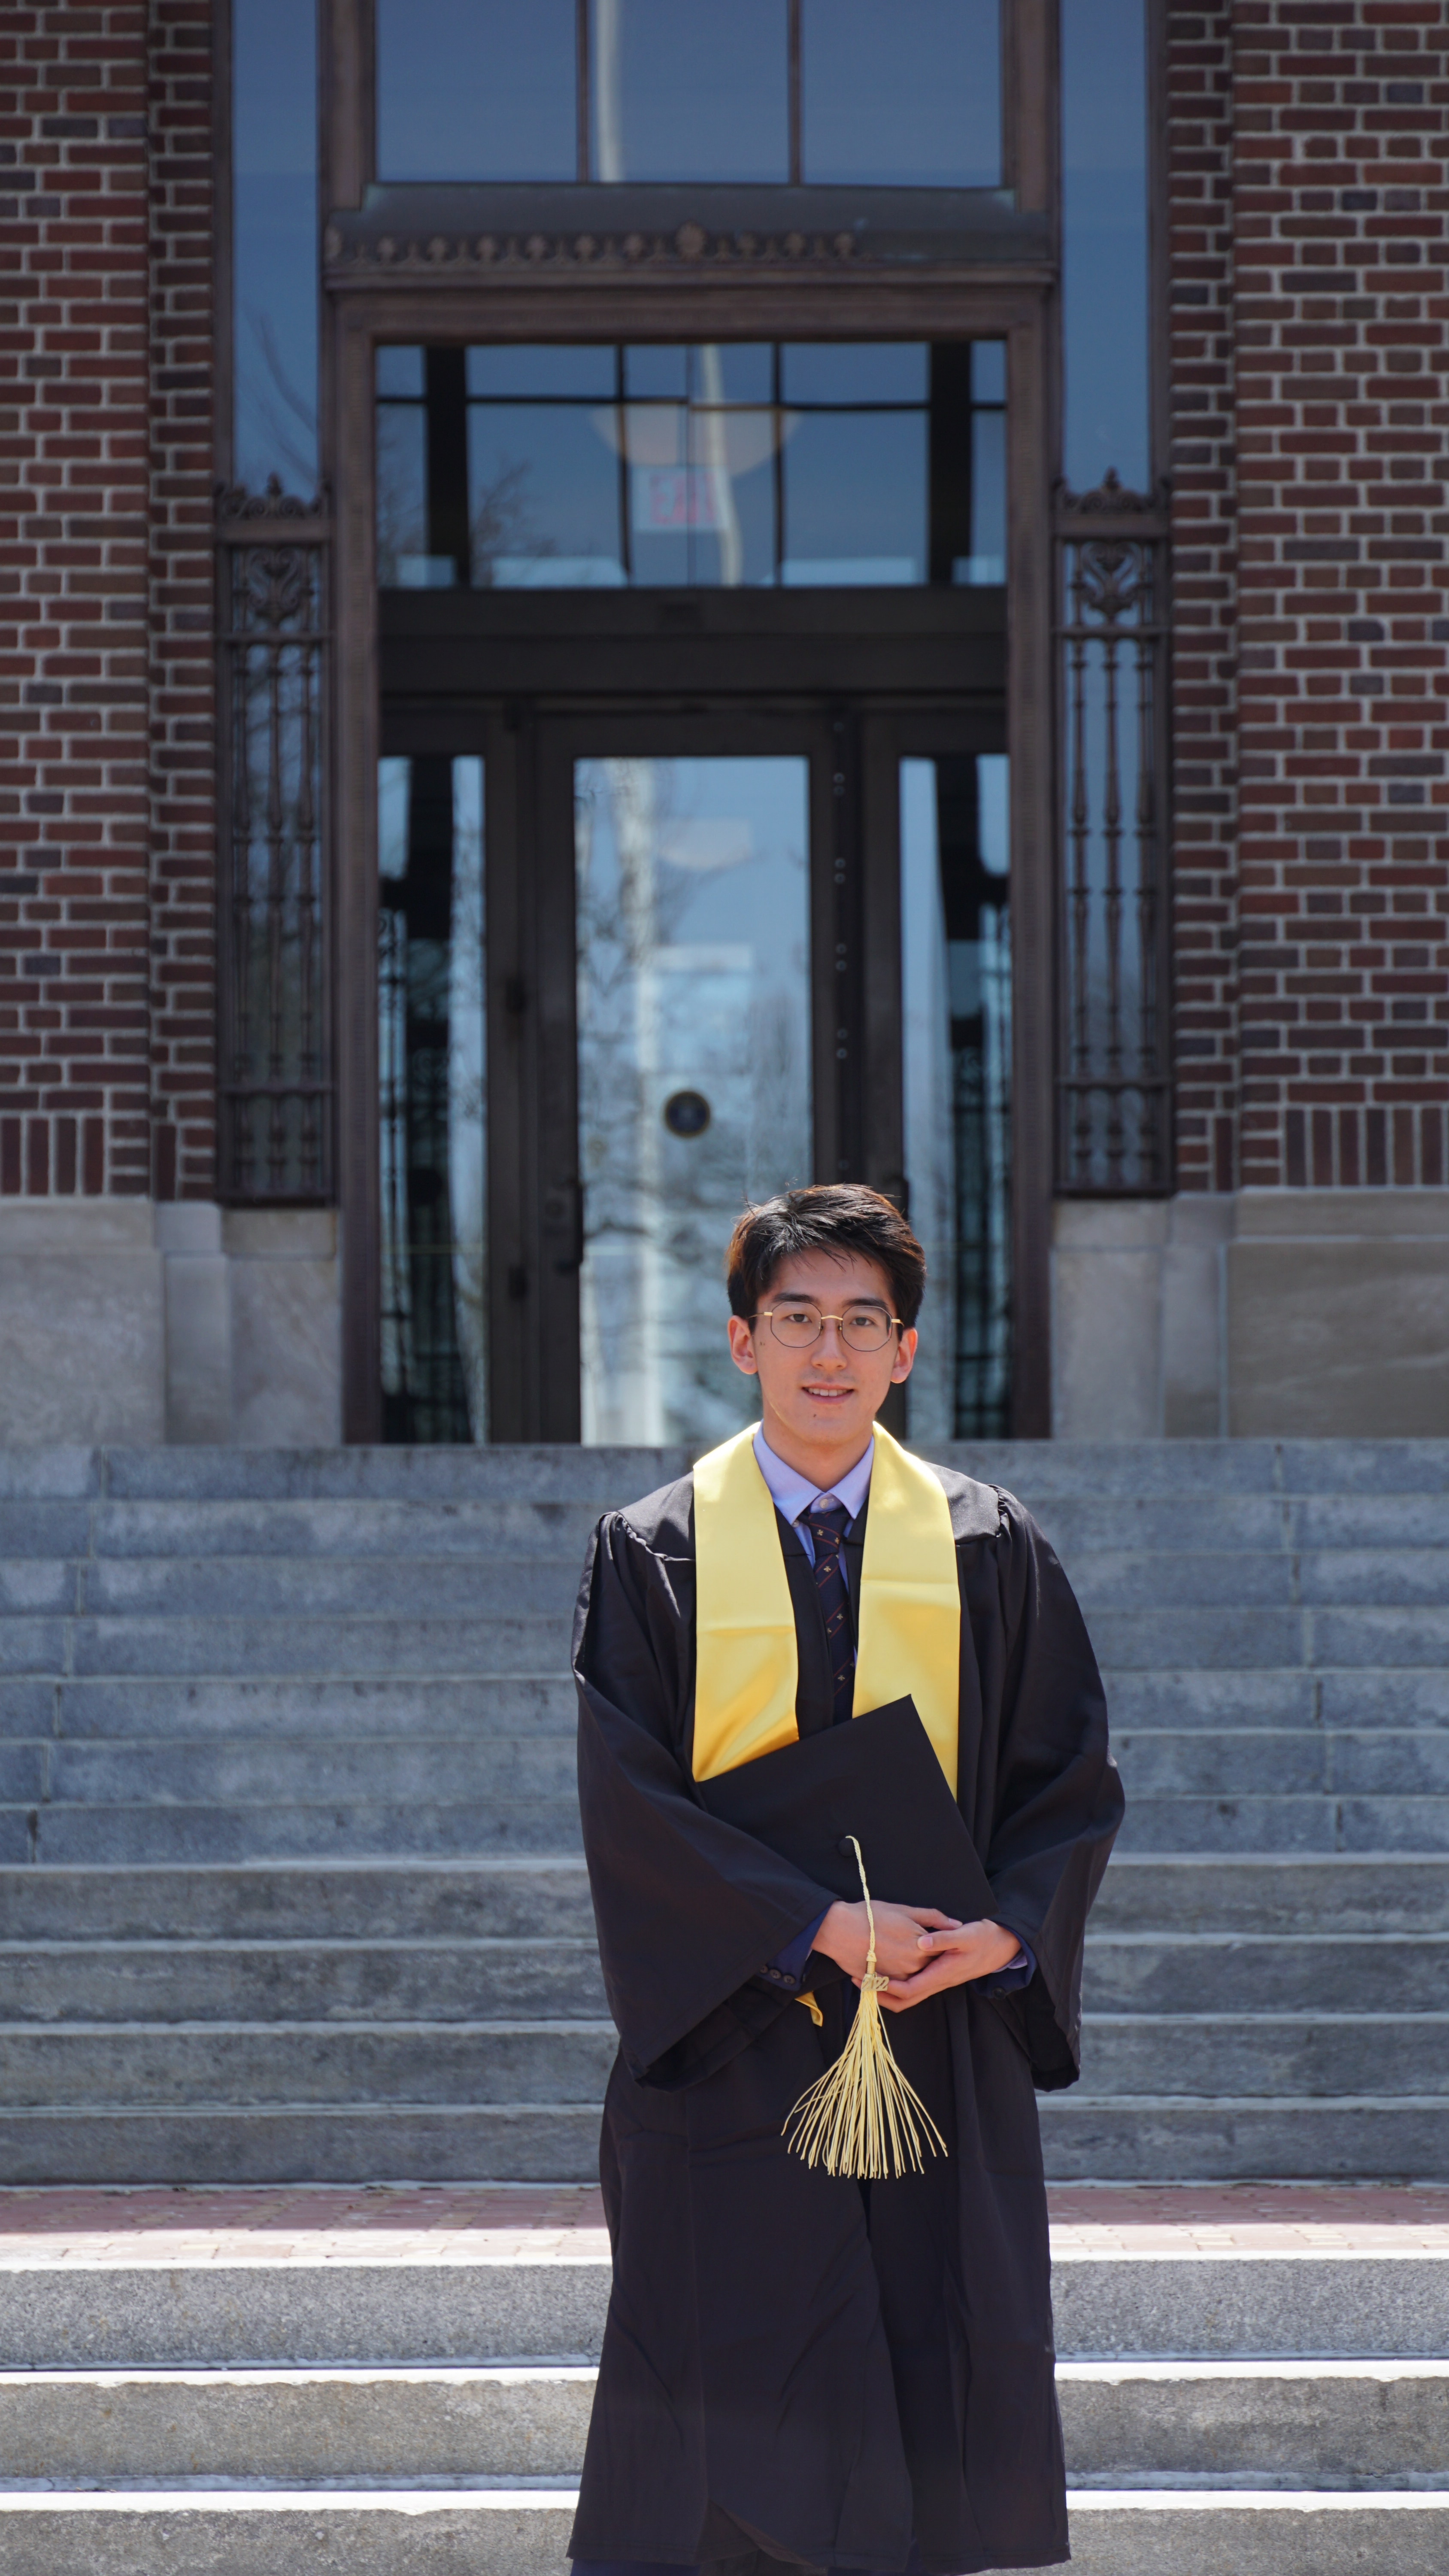
\includegraphics[width=0.5\textwidth,height=\textheight]{DSC00610.JPG}

\textbf{My favorite quote}
\textgreater{} ``All models are wrong, but some are useful''\\
\textgreater{} George E.P. Box

\textbf{Interests and Hobbies}
- I spent the first 18 years of my life in Shanghai, but I also lived in Boston for two years before coming to Ann Arbor, MI.
- In my free time I like to play tennis. I'm currently trying to improve my backhand and serving.
- I'm a big fan of electronic music. My most favorite genres are techno house, future house, future bass.
- My favorite novel is Neuromancer by William Gibson.
- I'm a coffee enthusiast. My favorite kind of coffee bean is Panama Geisha. If you happen to go to any coffee shop that is offering Geisha I highly recommend you to try it.

\textbf{More about Me\ldots{}}
You can find more information about my professional experiences on \href{https://www.linkedin.com/in/ycg2022/}{LinkedIn} and check out my past coding projects on \href{https://github.com/Yuchen-G}{Github}.

\hypertarget{nikita-mamidi}{%
\section{Nikita Mamidi}\label{nikita-mamidi}}

\textbf{I'm Nikita Mamidi 😃}

\begin{center}\rule{0.5\linewidth}{0.5pt}\end{center}


\includegraphics[width=9.375in,height=4.6875in]{nikita1.png}

\textbf{A little bit about me:}

I graduated from the University of Illinois at Urbana Champaign with a BS in Econometrics and Quantitative Economics. I look back fondly on my undergrad days where I was an Ambassador for the amazing Economics department, the Head Teaching Assistant for a Business Statistics Course and a Senior Associate at Illinois Business Consulting. \textbf{GO ILLINI!}

In today's world organizations are coming up with so many fascinating data and tech driven solutions to previously insurmountable problems. I want to be part of such a force that impacts the world positively. To achieve those high-level data science skills, I recently started my Masters of Business Analytics at the Ross School of Business!

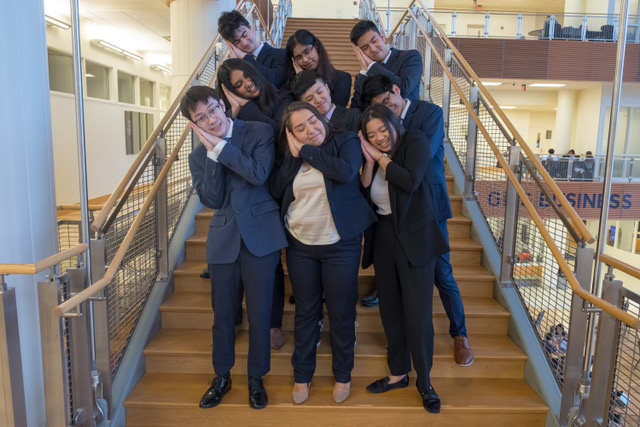
\includegraphics[width=4.6875in,height=3.64583in]{nikita3.jpeg} 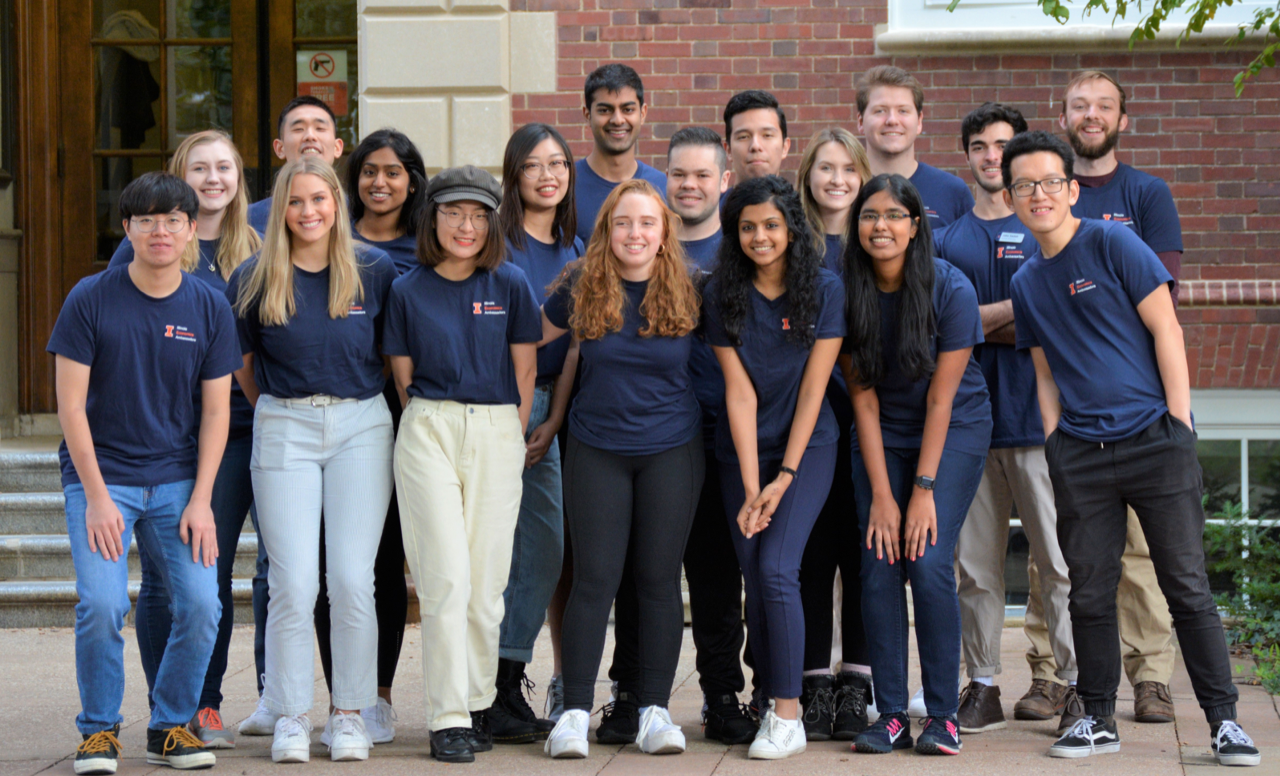
\includegraphics[width=4.6875in,height=3.64583in]{nikita2.png}

\begin{center}\rule{0.5\linewidth}{0.5pt}\end{center}

\textbf{Recent Work Experience:}

MSN Pharmaceuticals :- Sales and Marketing Executive

\begin{itemize}
\tightlist
\item
  Responsible for the South Korean, Japanese, Indonesian, Thailand and Taiwanese markets
\item
  Determined potential partnerships in East Asia, established contacts \& built relationships with key decision makers
\item
  Collaborated with technical teams to ensure production and distribution of high-quality samples and final API
\item
  Achieved the \textbf{\$3 million per month} revenue target for the past 2 quarters
\end{itemize}

\begin{center}\rule{0.5\linewidth}{0.5pt}\end{center}

\textbf{Fun Facts:}

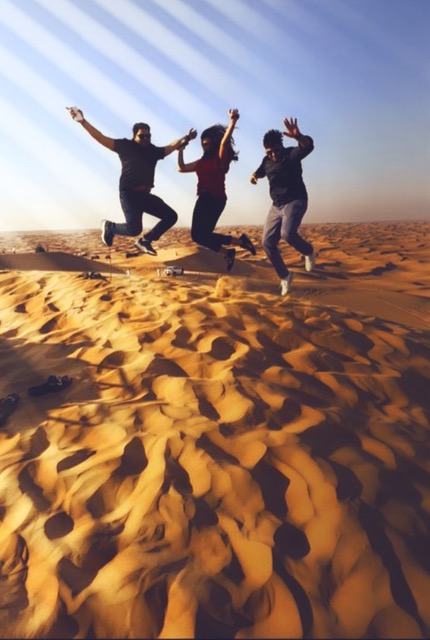
\includegraphics[width=3.33333in,height=3.64583in]{nikita4.jpeg} 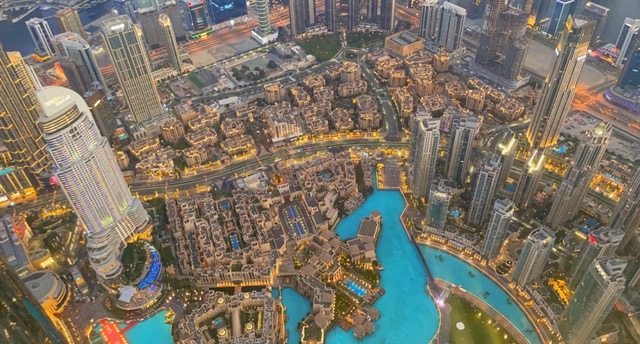
\includegraphics[width=5.20833in,height=3.64583in]{nikita5.jpeg}

\begin{itemize}
\tightlist
\item
  I love to travel. Been to 20 countries. Next Destination - Mexico 🇲🇽
\item
  Stock market trading is everything! I'm a day trader tho, I know I'm awful 🤭
\item
  Certified online shopaholic. But I also return the goods with equal speed
\item
  I love watching (and dreaming of playing) in the NBA
\item
  I enjoy snorkeling and scuba diving
\item
  I'm terrified of all animals. Yes, including cute puppies and kittens 🤯
\end{itemize}

\textbf{That's enough about me 😁. Please reach out so I can learn more about You!}

\href{https://www.linkedin.com/in/nikita-mamidi-763b80185/}{Linkedin}

Contact - 217-898-6828

\hypertarget{ben-newman}{%
\section{Ben Newman}\label{ben-newman}}

\begin{quote}
Team: Coded in COBOL
\end{quote}

Bio: Hi, I'm Ben. I was raised in Midland, MI. It's in the middle-right part of the mitten. In high school, I was on the swim team (see below) and did cross country. I also attended University of Michigan from which I graduated last year (see below). Some things that bring joy to my life are friends, family, my pets (see below), skiing, fishing, and going to Michigan Football Games!!

\textbf{My Education}

\begin{itemize}
\tightlist
\item
  Saint Brigid Catholic School (Midland, MI USA)
\item
  Herbert Henry Dow High School (Midland, MI USA)
\item
  University of Michigan Ann Arbor (Ann Arbor, MI USA)

  \begin{itemize}
  \tightlist
  \item
    B.S. Statistics
  \end{itemize}
\item
  University of Michigan Ann Arbor (Ann Arbor, MI USA)

  \begin{itemize}
  \tightlist
  \item
    Masters in Business Analytics
  \end{itemize}
\end{itemize}

\textbf{My favorite foods.}

\begin{enumerate}
\def\labelenumi{\arabic{enumi}.}
\tightlist
\item
  Pizza
\item
  Orange Chicken
\item
  Burgers
\end{enumerate}

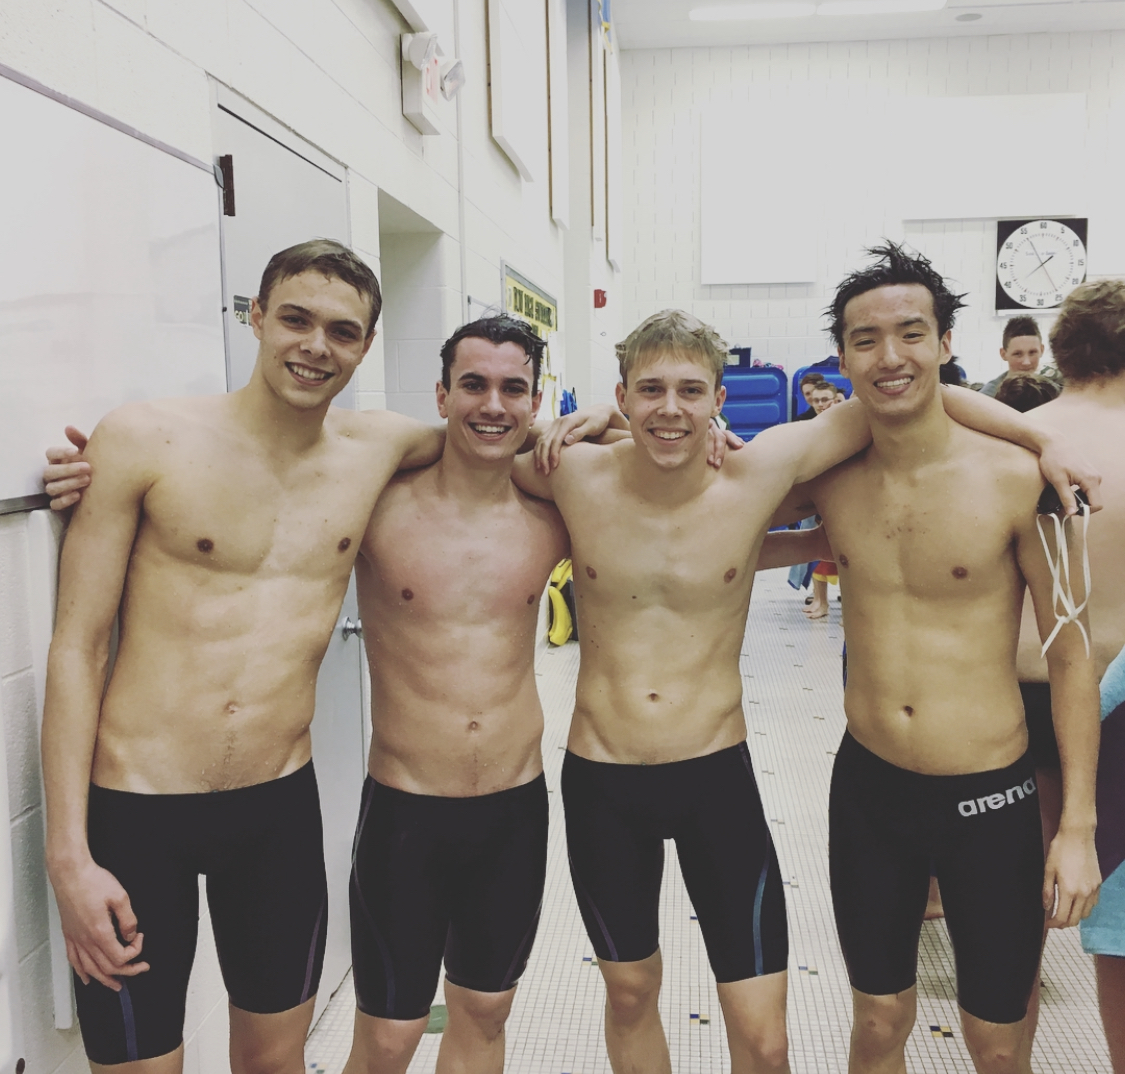
\includegraphics[width=0.25\textwidth,height=\textheight]{swimmers.jpg}

\begin{quote}
A picture of me (left) in my more fit days on the swim team (circa 2017).
\end{quote}

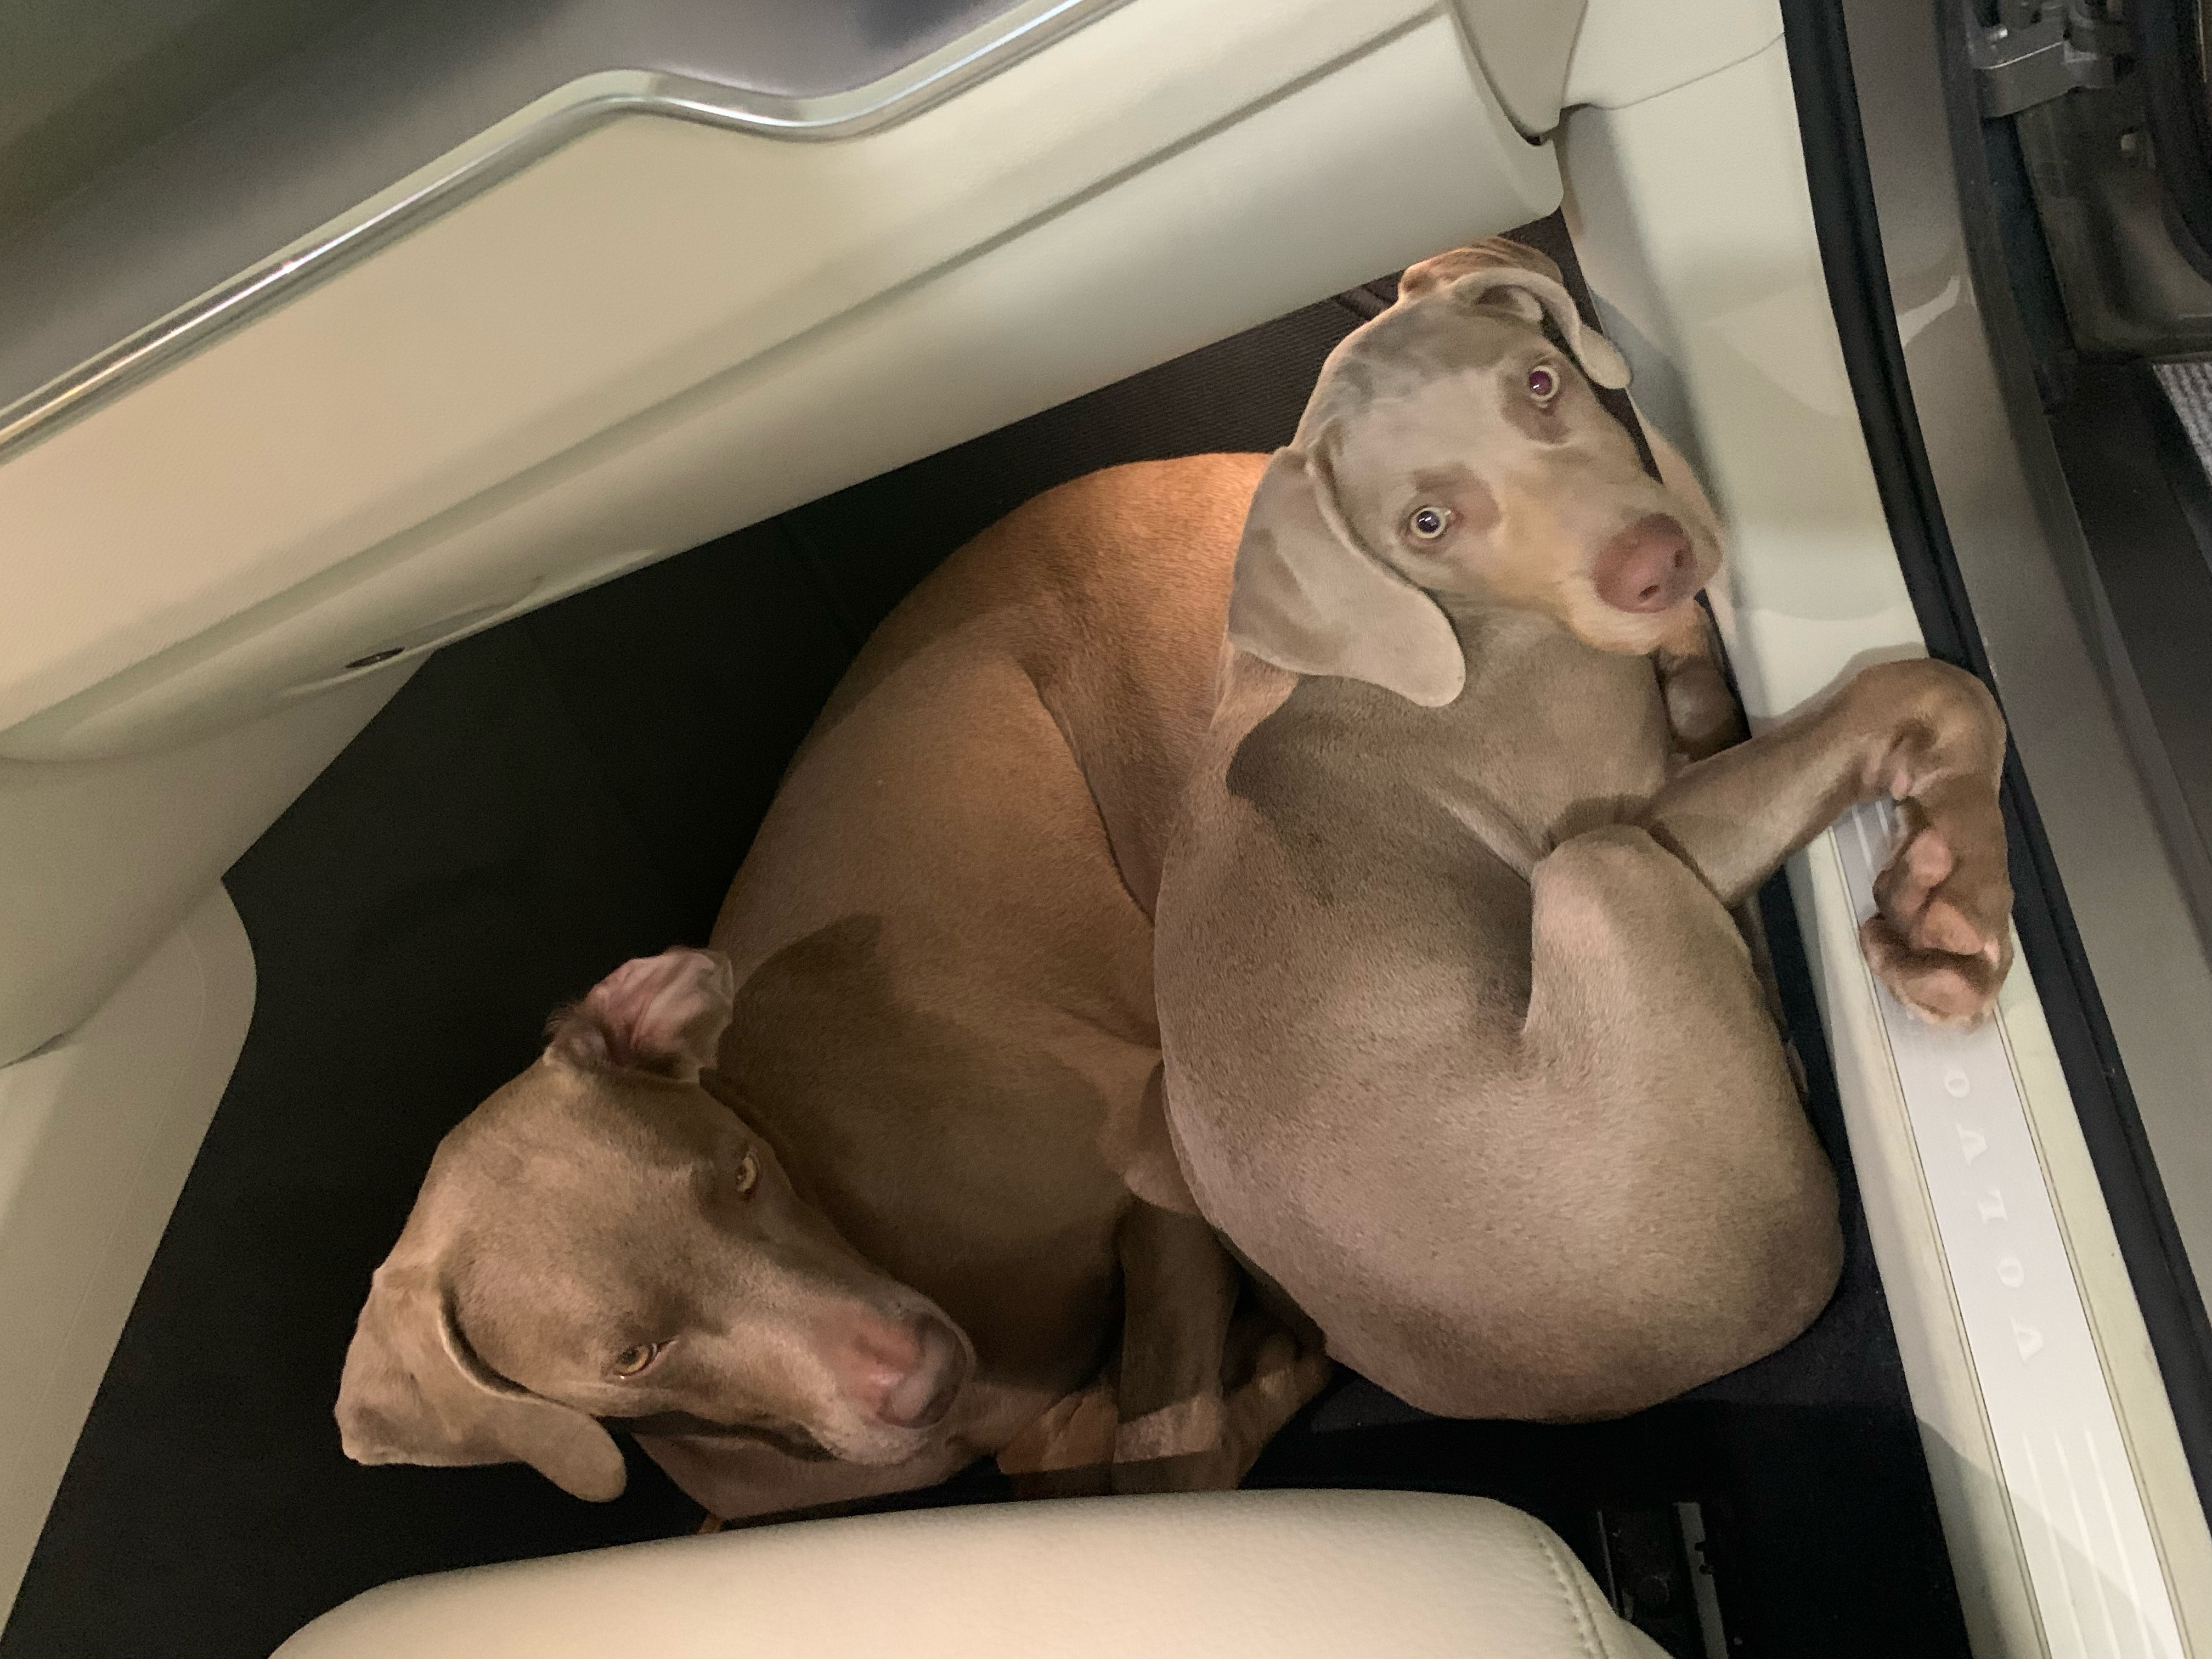
\includegraphics[width=0.25\textwidth,height=\textheight]{dogs.jpeg}

\begin{quote}
A picture of my dogs Pearl (left) and Blue (right). They are Weimaraners.
\end{quote}

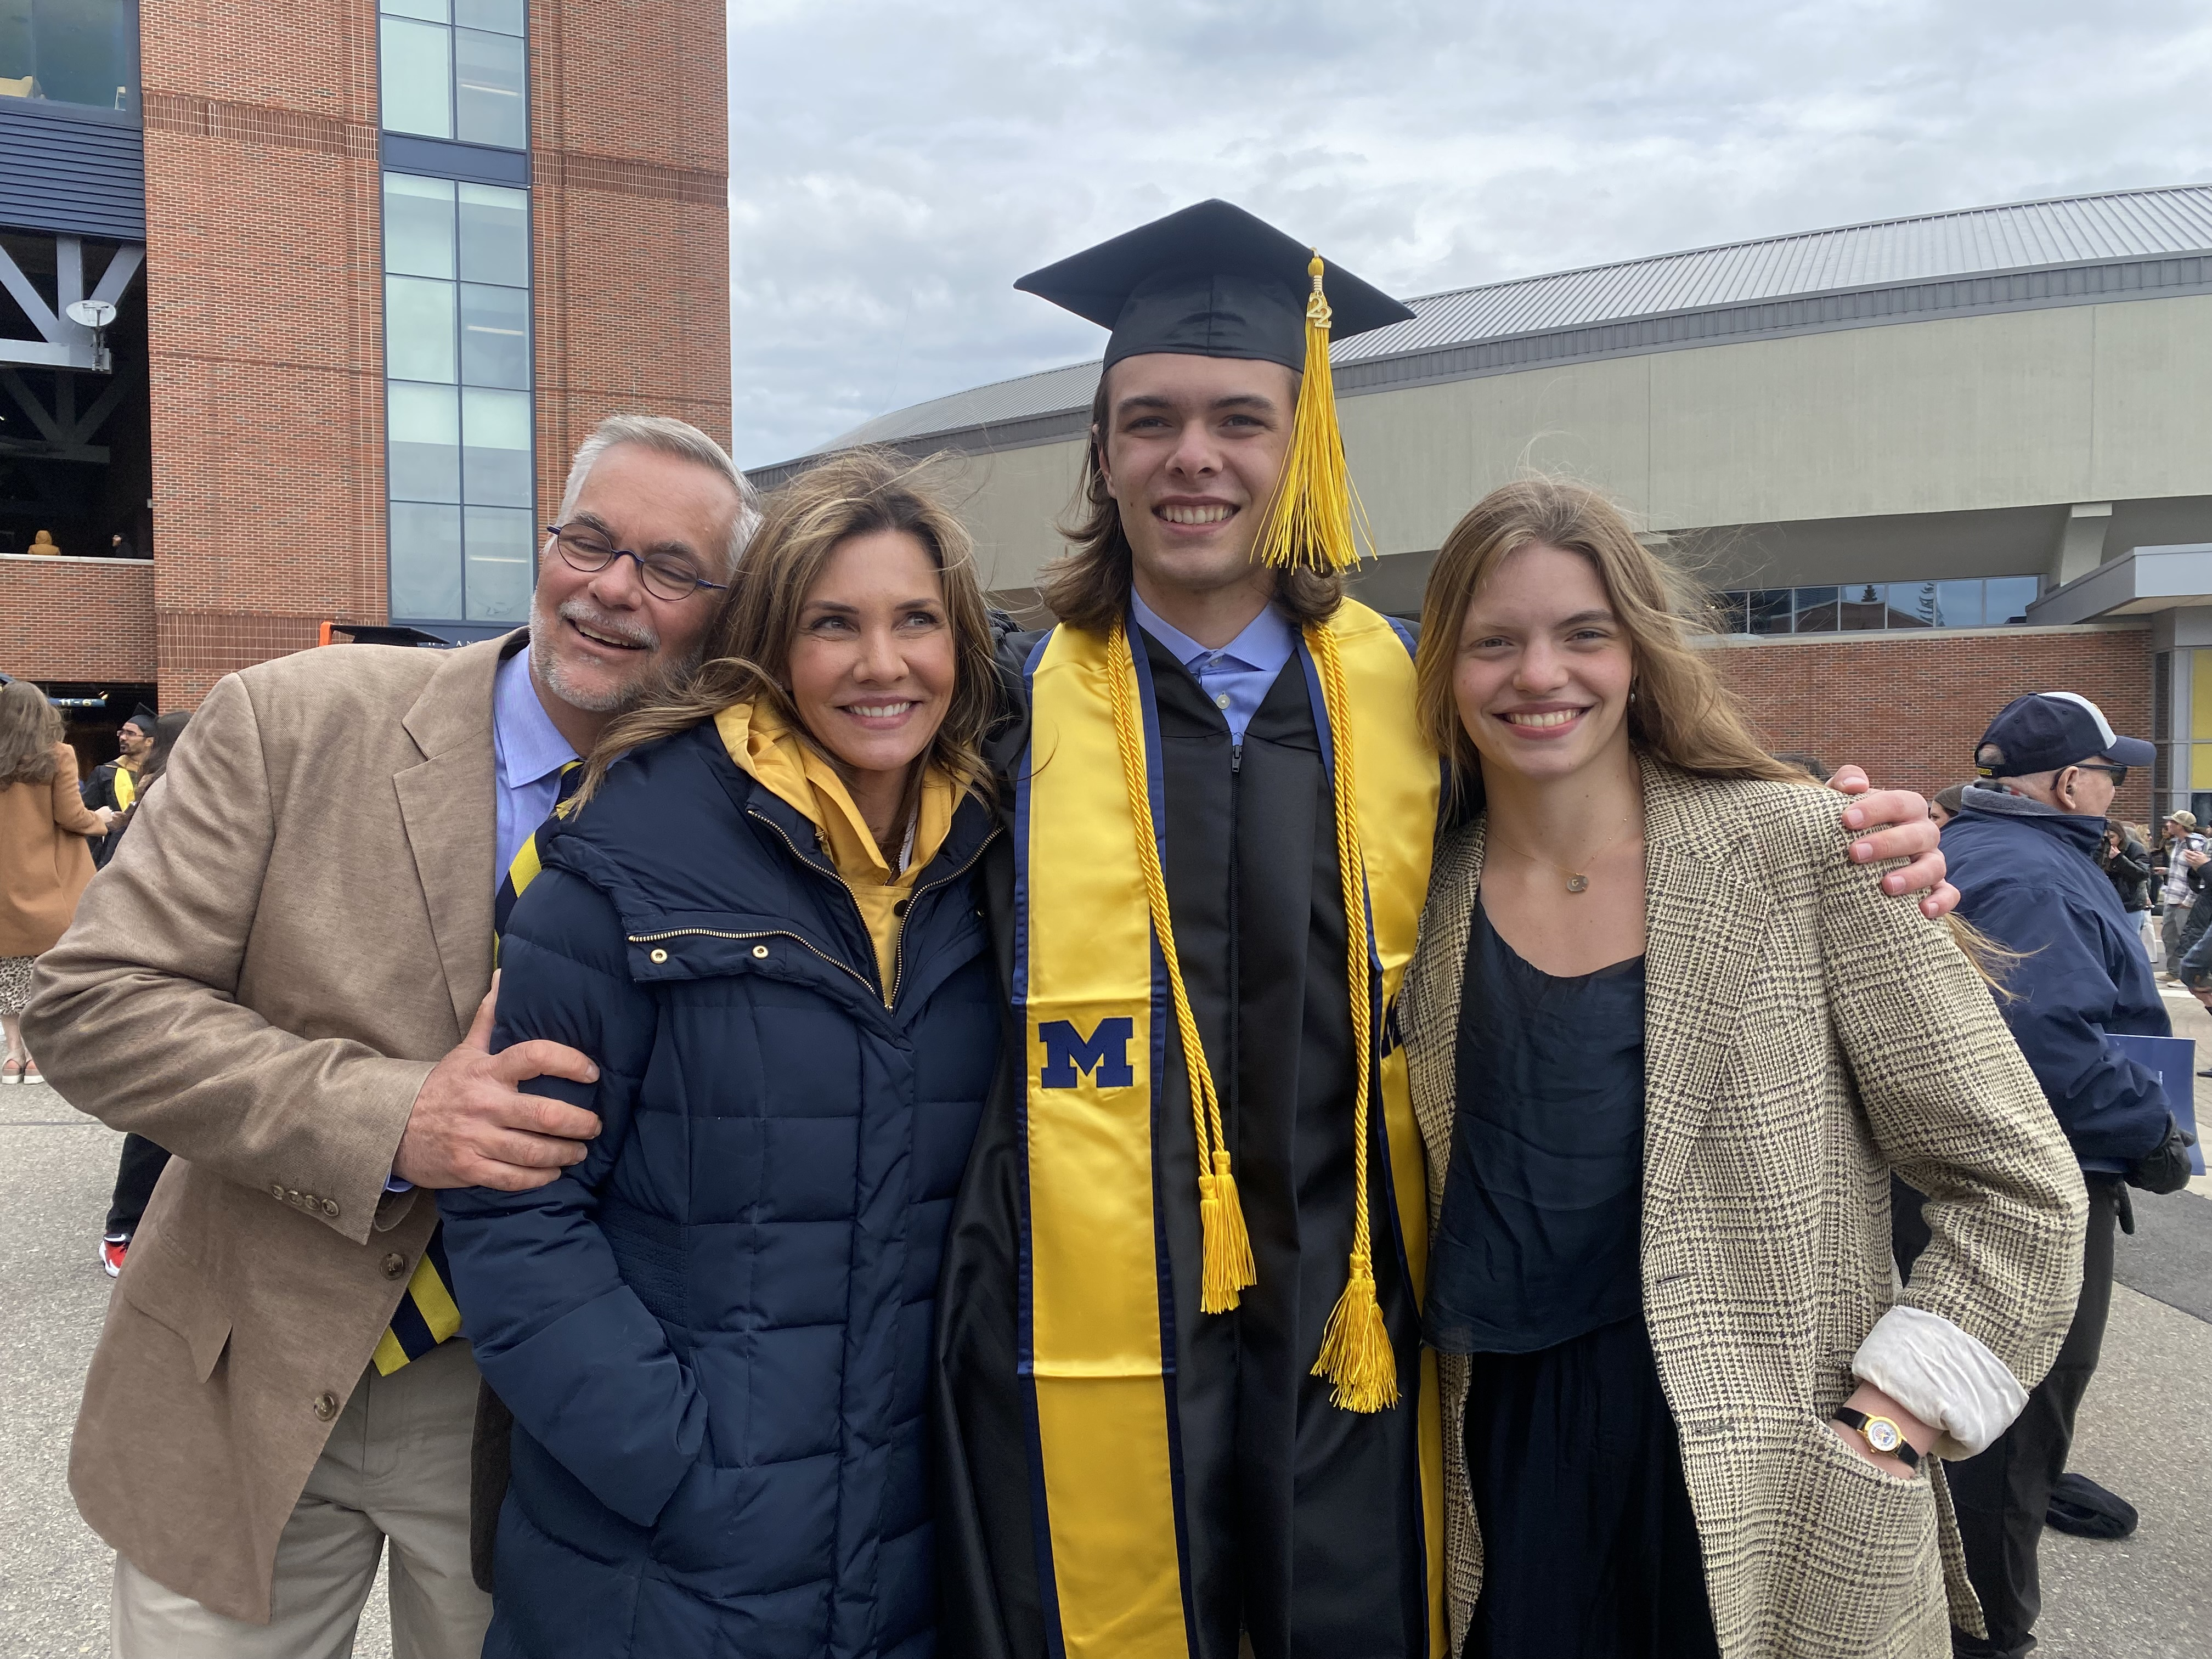
\includegraphics[width=0.25\textwidth,height=\textheight]{Graduation.jpg}

\begin{quote}
This is me at the University of Michigan Commencement with my family in April, 2022.
\end{quote}

\hypertarget{peiyue-sun}{%
\section{Peiyue Sun}\label{peiyue-sun}}

This is Peiyue Sun.

\begin{itemize}
\tightlist
\item
  I love Michigan Wolverines!
\item
  I love Wisconsin Badgers!
\end{itemize}

Education:

\begin{itemize}
\tightlist
\item
  Wisconsin School of Business 2016 -\textgreater{} 2019 Risk Management \& Insurance (BBA)
\item
  Ross School of Business 2022 -\textgreater{} 2023 Business Analytics (MBAn)
\end{itemize}

Technology used:

\begin{itemize}
\tightlist
\item
  R
\item
  Python
\item
  Excel
\end{itemize}

Work Experience:

\begin{itemize}
\tightlist
\item
  2 years at Willis Towers Watson risk consulting sector

  \begin{itemize}
  \tightlist
  \item
    Insurance-linked securities valuation
  \item
    Financial Reserving for global insurance enterprises
  \end{itemize}
\end{itemize}

Goal at MBAN:

\begin{itemize}
\tightlist
\item
  Unlock my potential in business analytics and project management
\end{itemize}

Hobbies:

\begin{itemize}
\tightlist
\item
  Snooker, Basketball, Texas Hold'em, Swimming, Running, Biking, and Trap music festivals
\end{itemize}

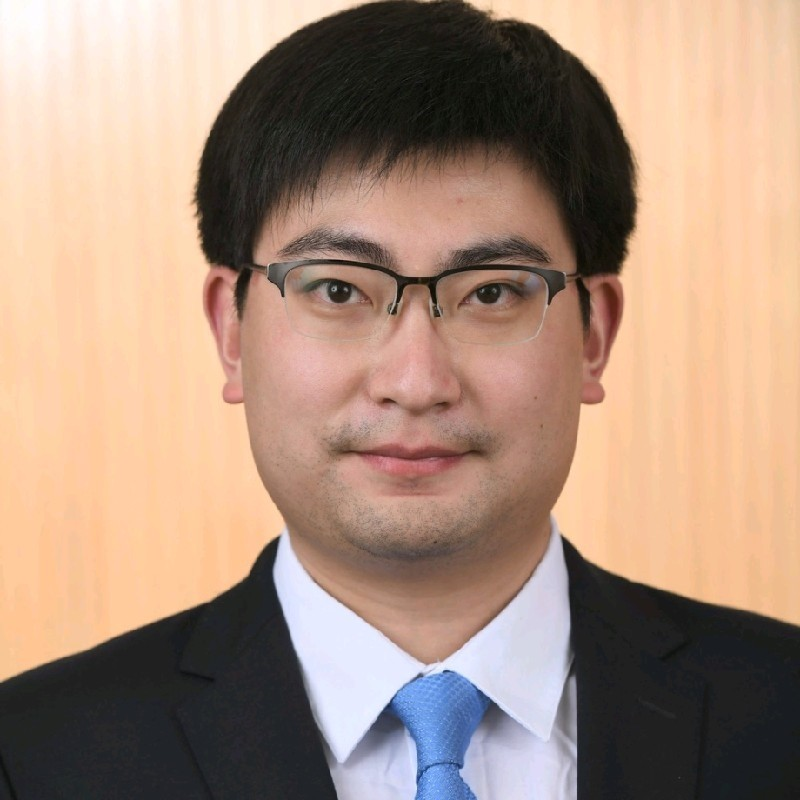
\includegraphics[width=2.66667in,height=\textheight]{1.jpg}

\hypertarget{winnifer-chen}{%
\section{Winnifer Chen}\label{winnifer-chen}}

Winnifer Chen

Email: \href{mailto:winnifer@umich.edu}{\nolinkurl{winnifer@umich.edu}}

Phone: (980) 298-7184

LinkedIn: \url{https://www.linkedin.com/in/winnifer/}

\textbf{Educational Background}

I recently graduated with a Bachelor of Science in Economics with a minor in Statistics from the University of Michigan in April 2022. Currently, I am pursuing a Master of Business Analytics at the University of Michigan - Stephen M. Ross School of Business, with an expected graduation date of April 2023.

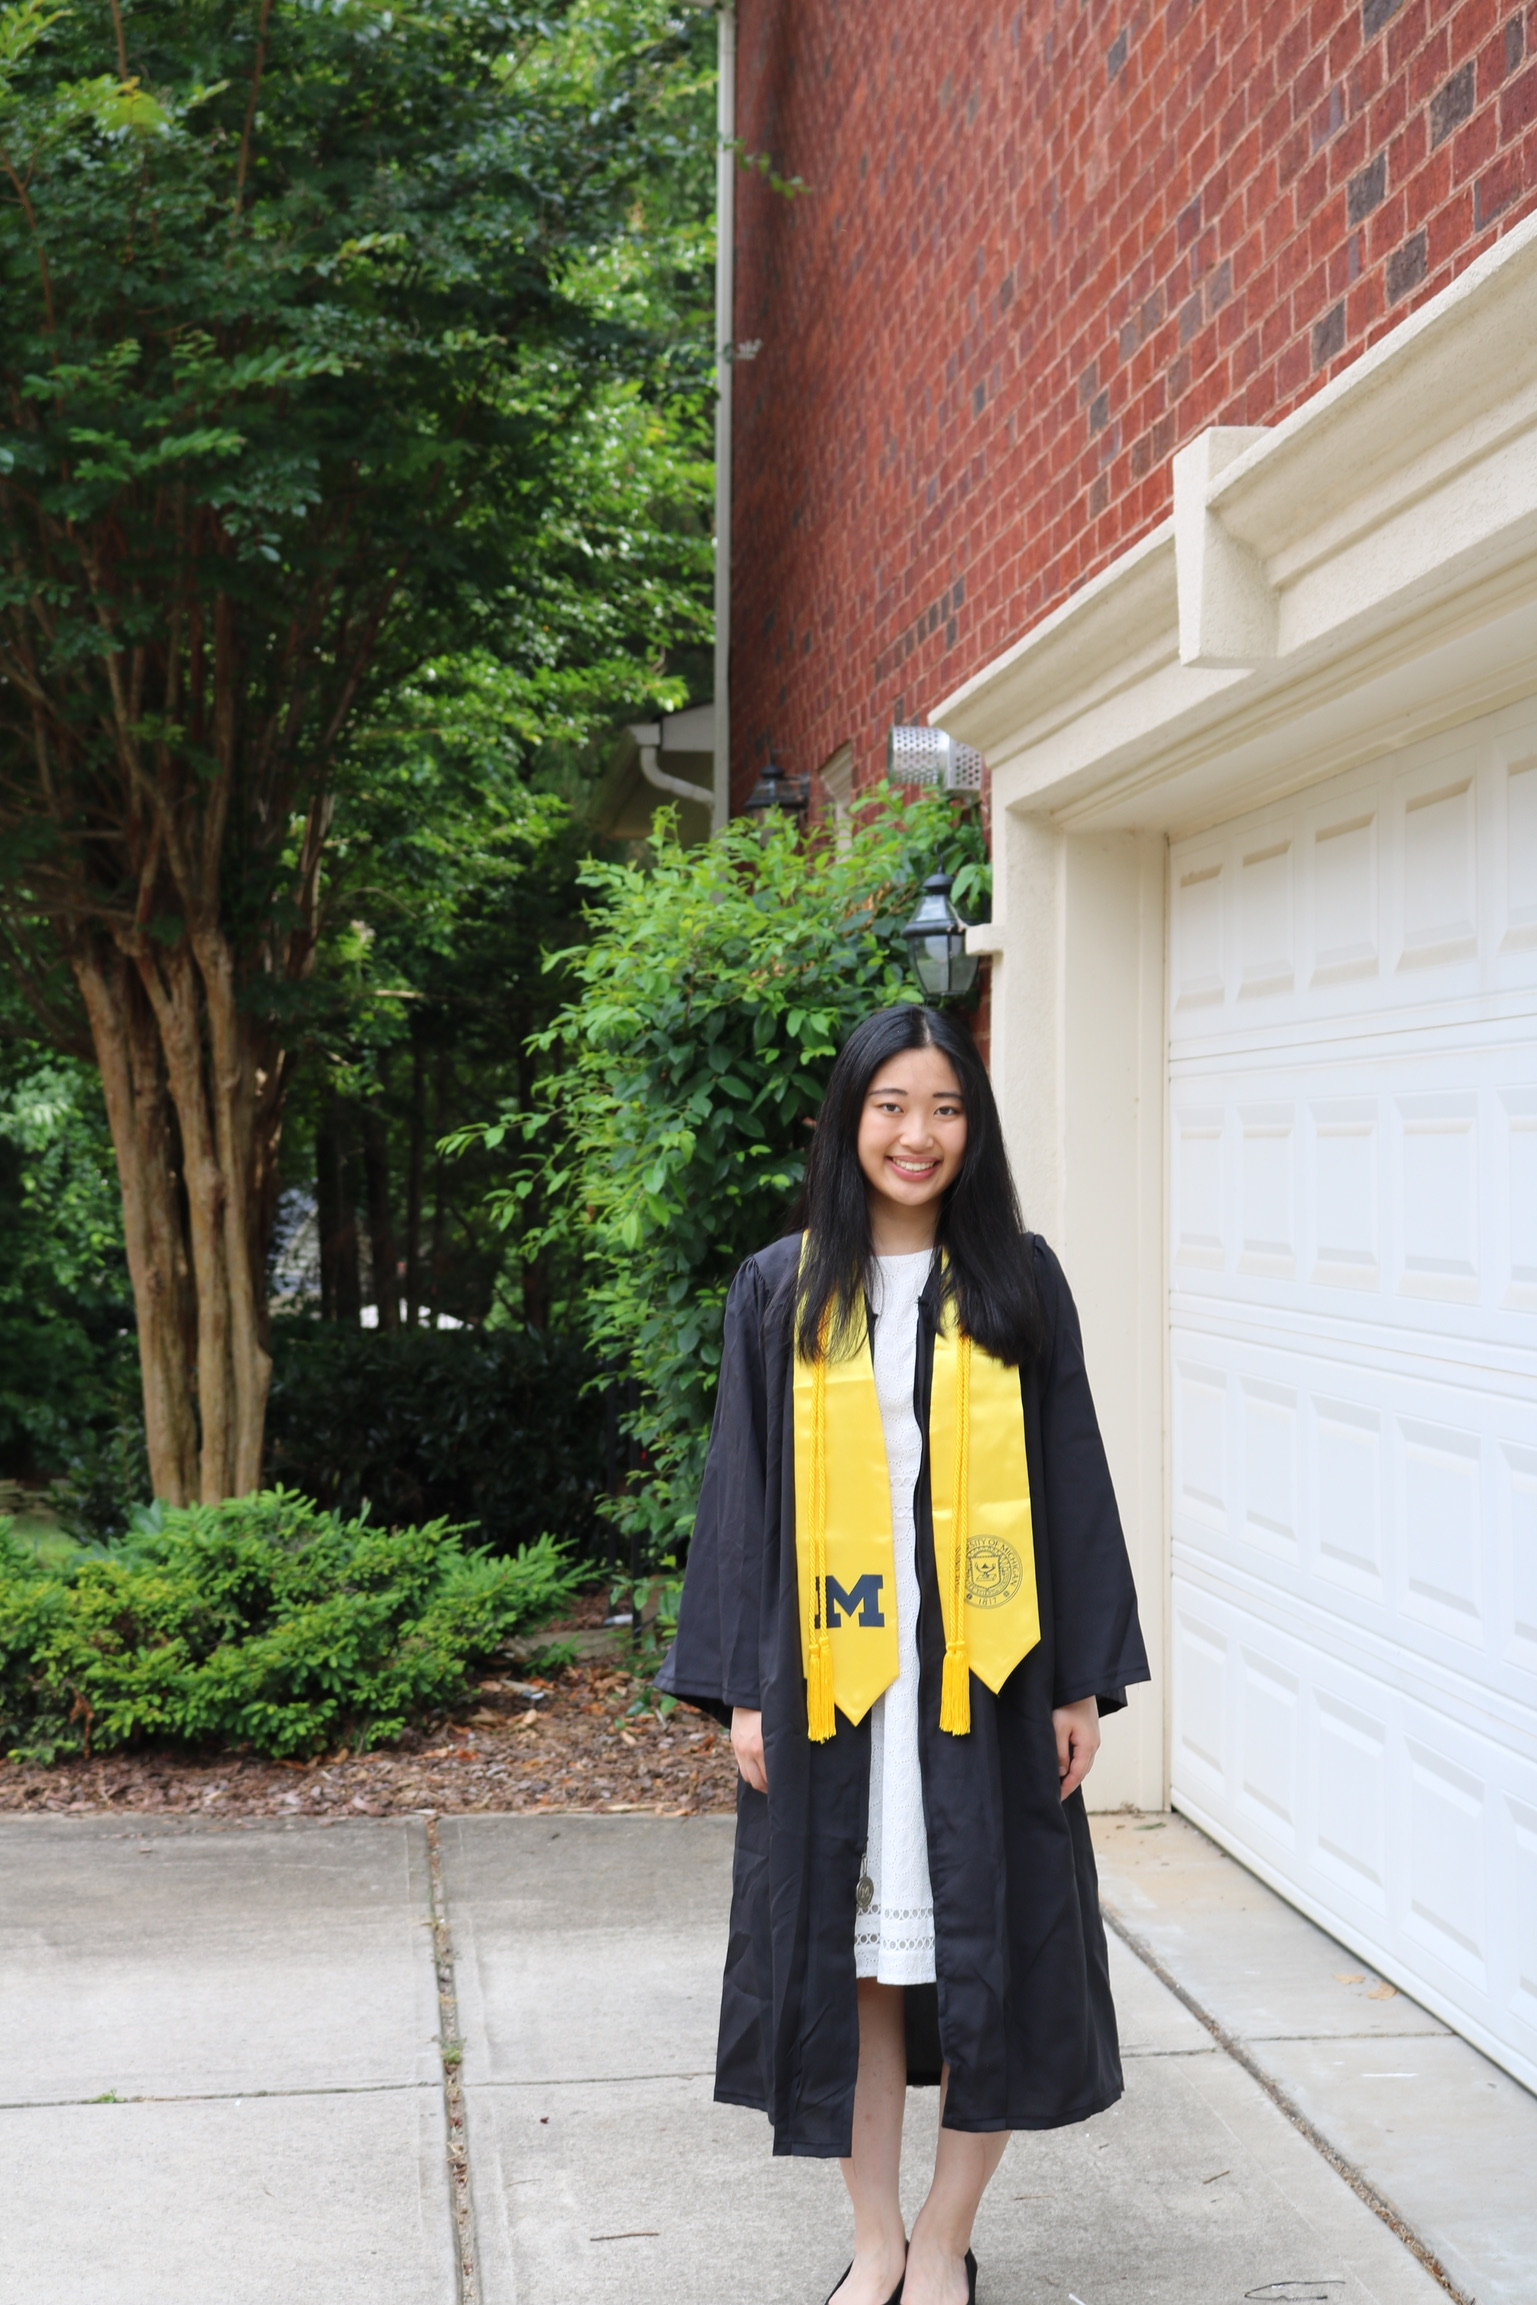
\includegraphics[width=0.25\textwidth,height=\textheight]{grad.JPG}
\includegraphics[width=0.4\textwidth,height=\textheight]{fam.JPG}
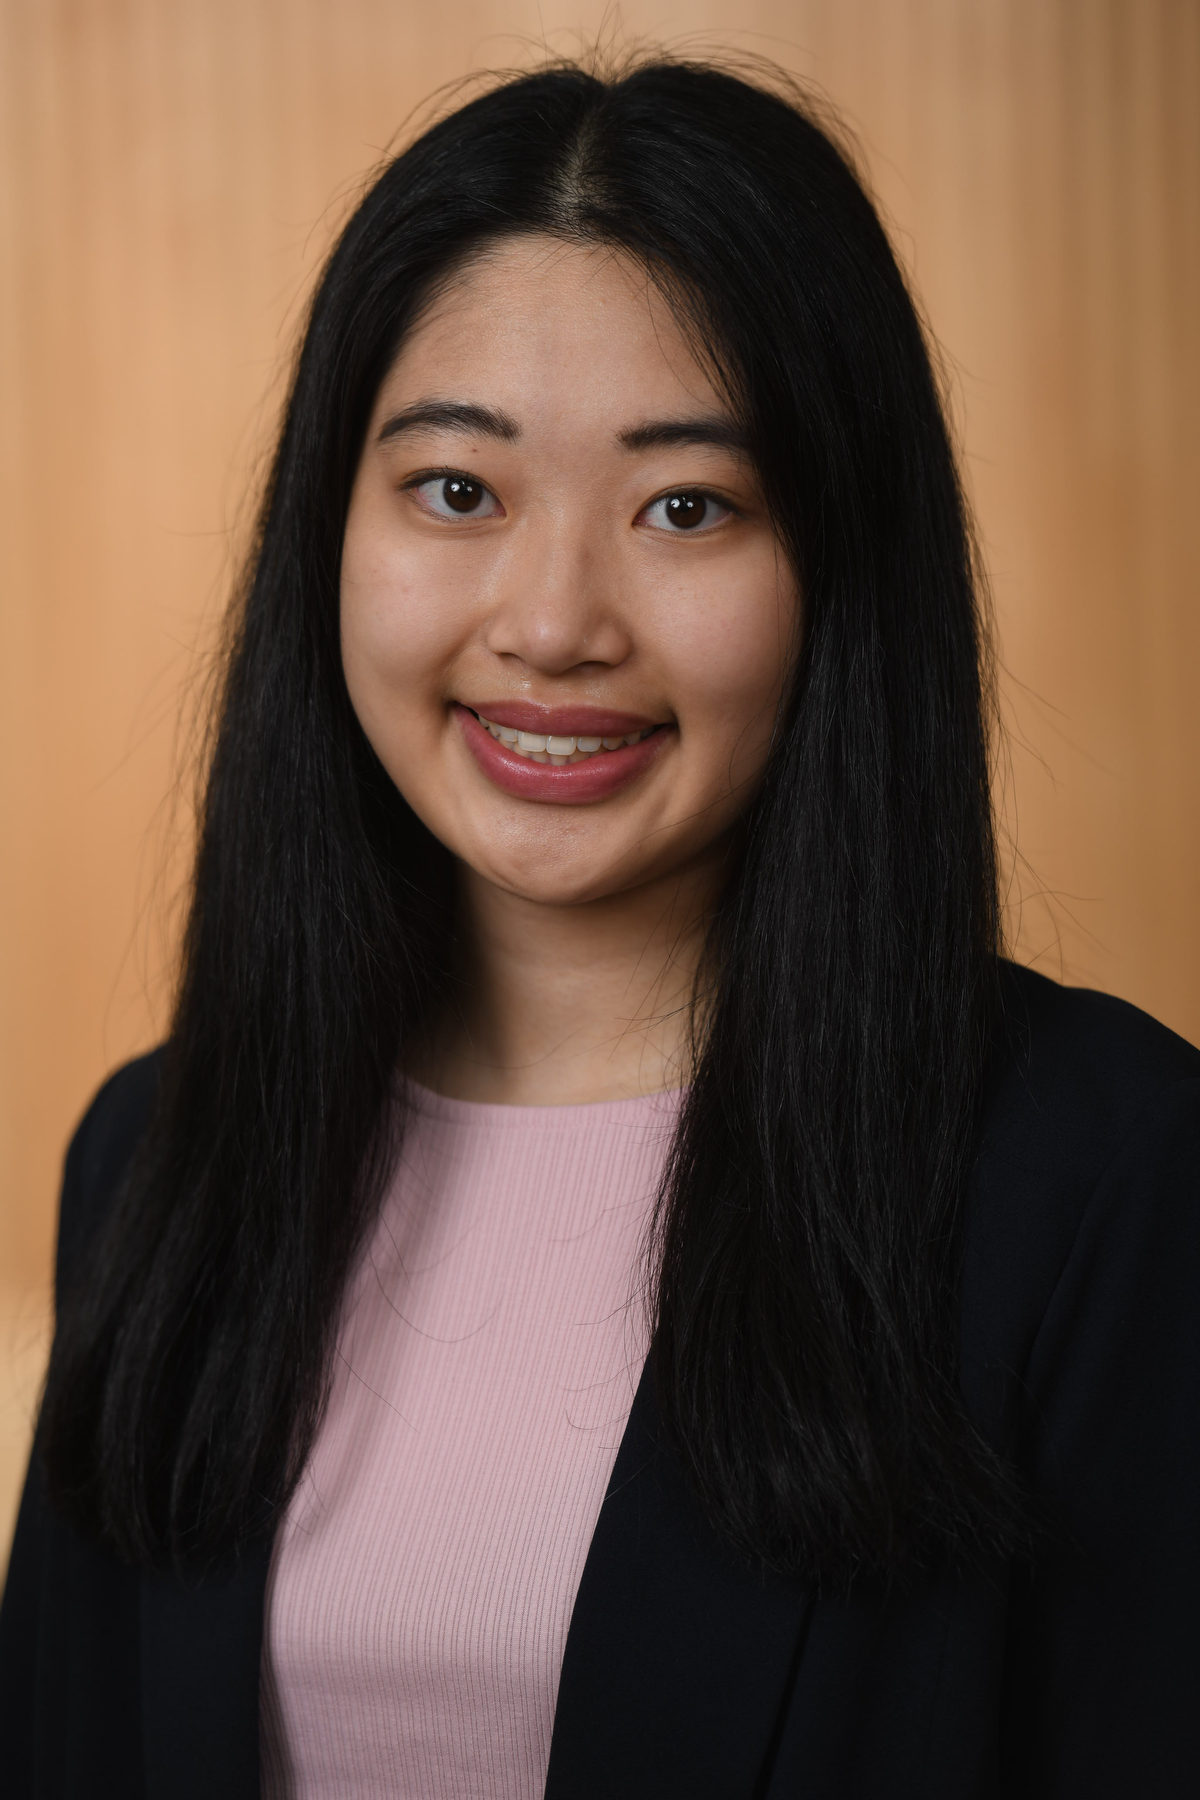
\includegraphics[width=0.25\textwidth,height=\textheight]{headshot.jpg}

\textbf{Fun Facts!}

\begin{itemize}
\tightlist
\item
  I am from Ann Arbor, MI, but throughout my life, I have also lived in Charlotte, NC and Taipei, Taiwan.
\item
  I come from a family of Wolverines! Both of my parents also attended graduate school at Michigan, and my younger sister is starting her freshman year this fall. GO BLUE!
\item
  In my free time, I love to spend time outdoors, whether that is hiking, camping, or taking pictures of scenery. Check out some of the pictures I took: \url{https://vsco.co/winniferchen/gallery}
\item
  I really enjoy rewatching music videos and performances by my favorite kpop groups. One of my dreams is to go to a kpop concert one day and sit in the very front section.
\item
  Immersing myself in the world of kdramas is another way for me to wind down and relax after a long day.
\item
  Something that I want to do more this year is trying new recipes and cooking more.
\end{itemize}

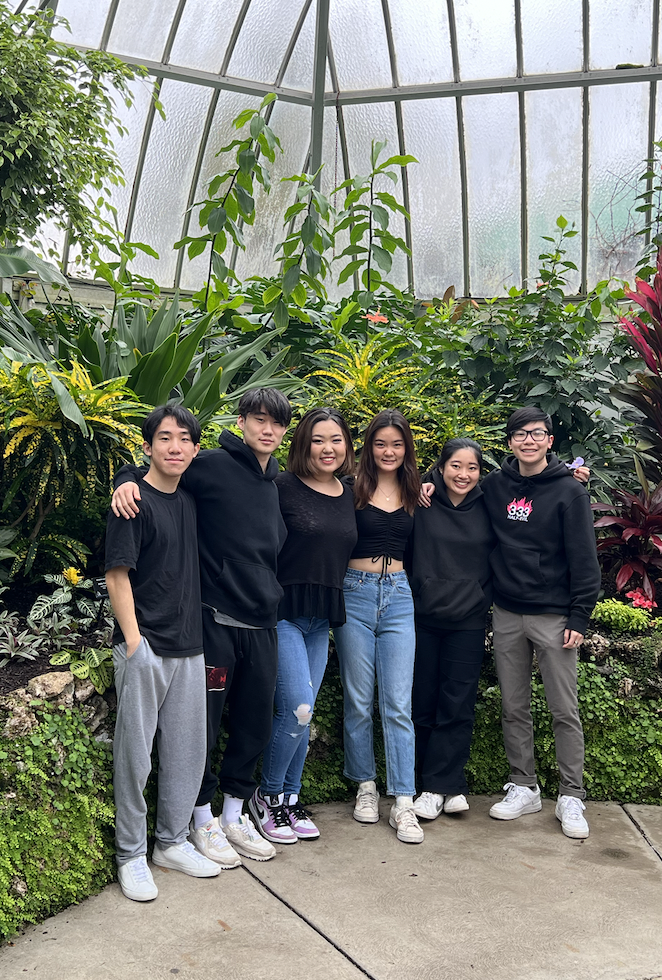
\includegraphics[width=0.23\textwidth,height=\textheight]{dtw.png}
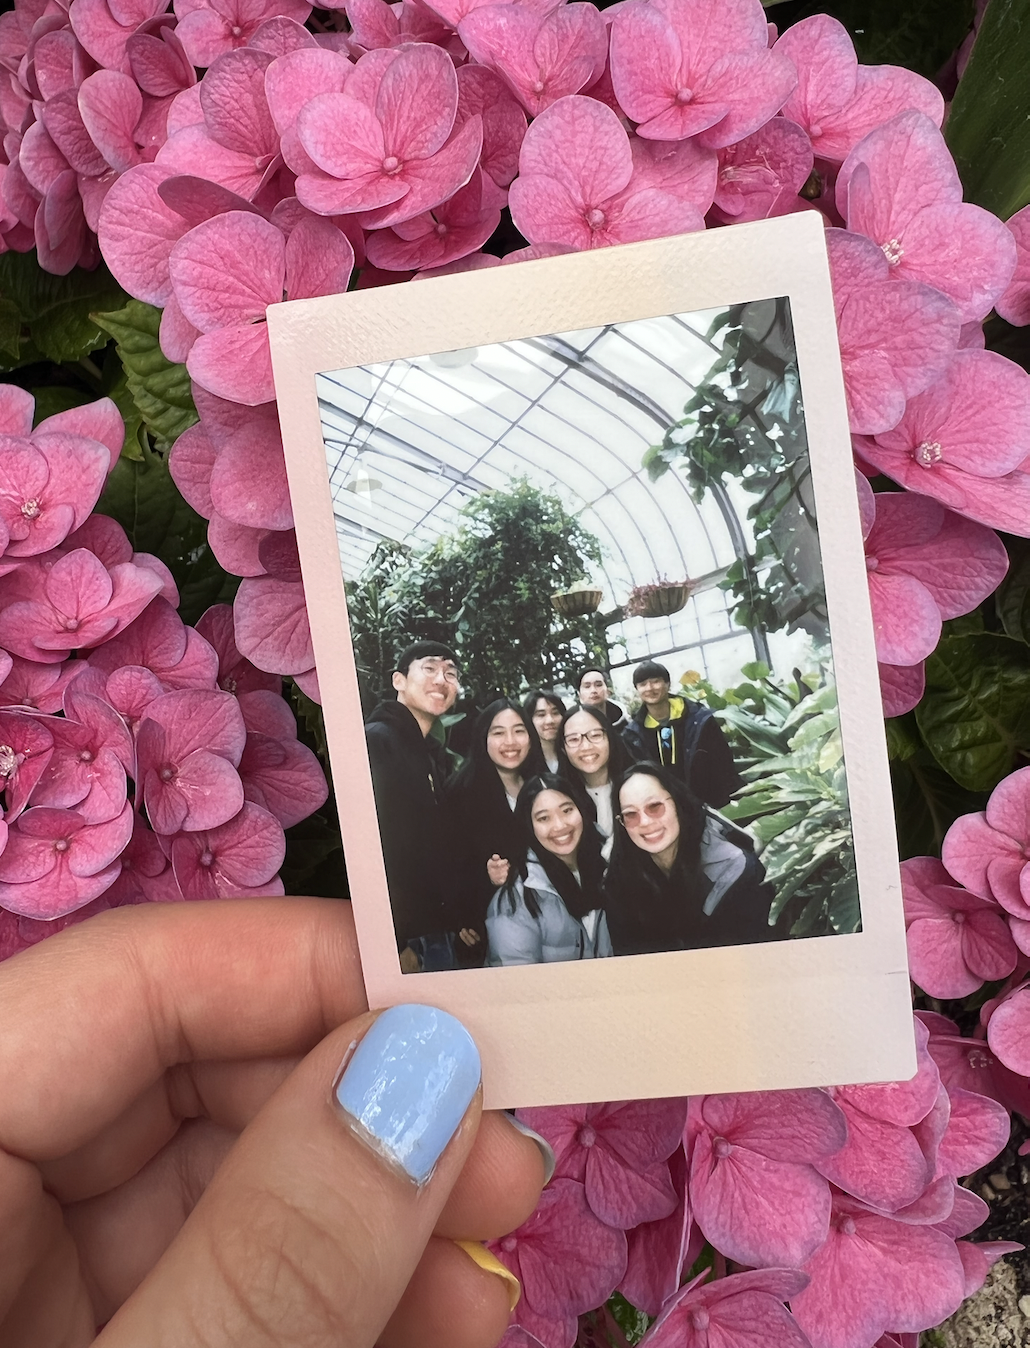
\includegraphics[width=0.25\textwidth,height=\textheight]{belleisle.png}

\includegraphics[width=0.25\textwidth,height=\textheight]{econ.png}
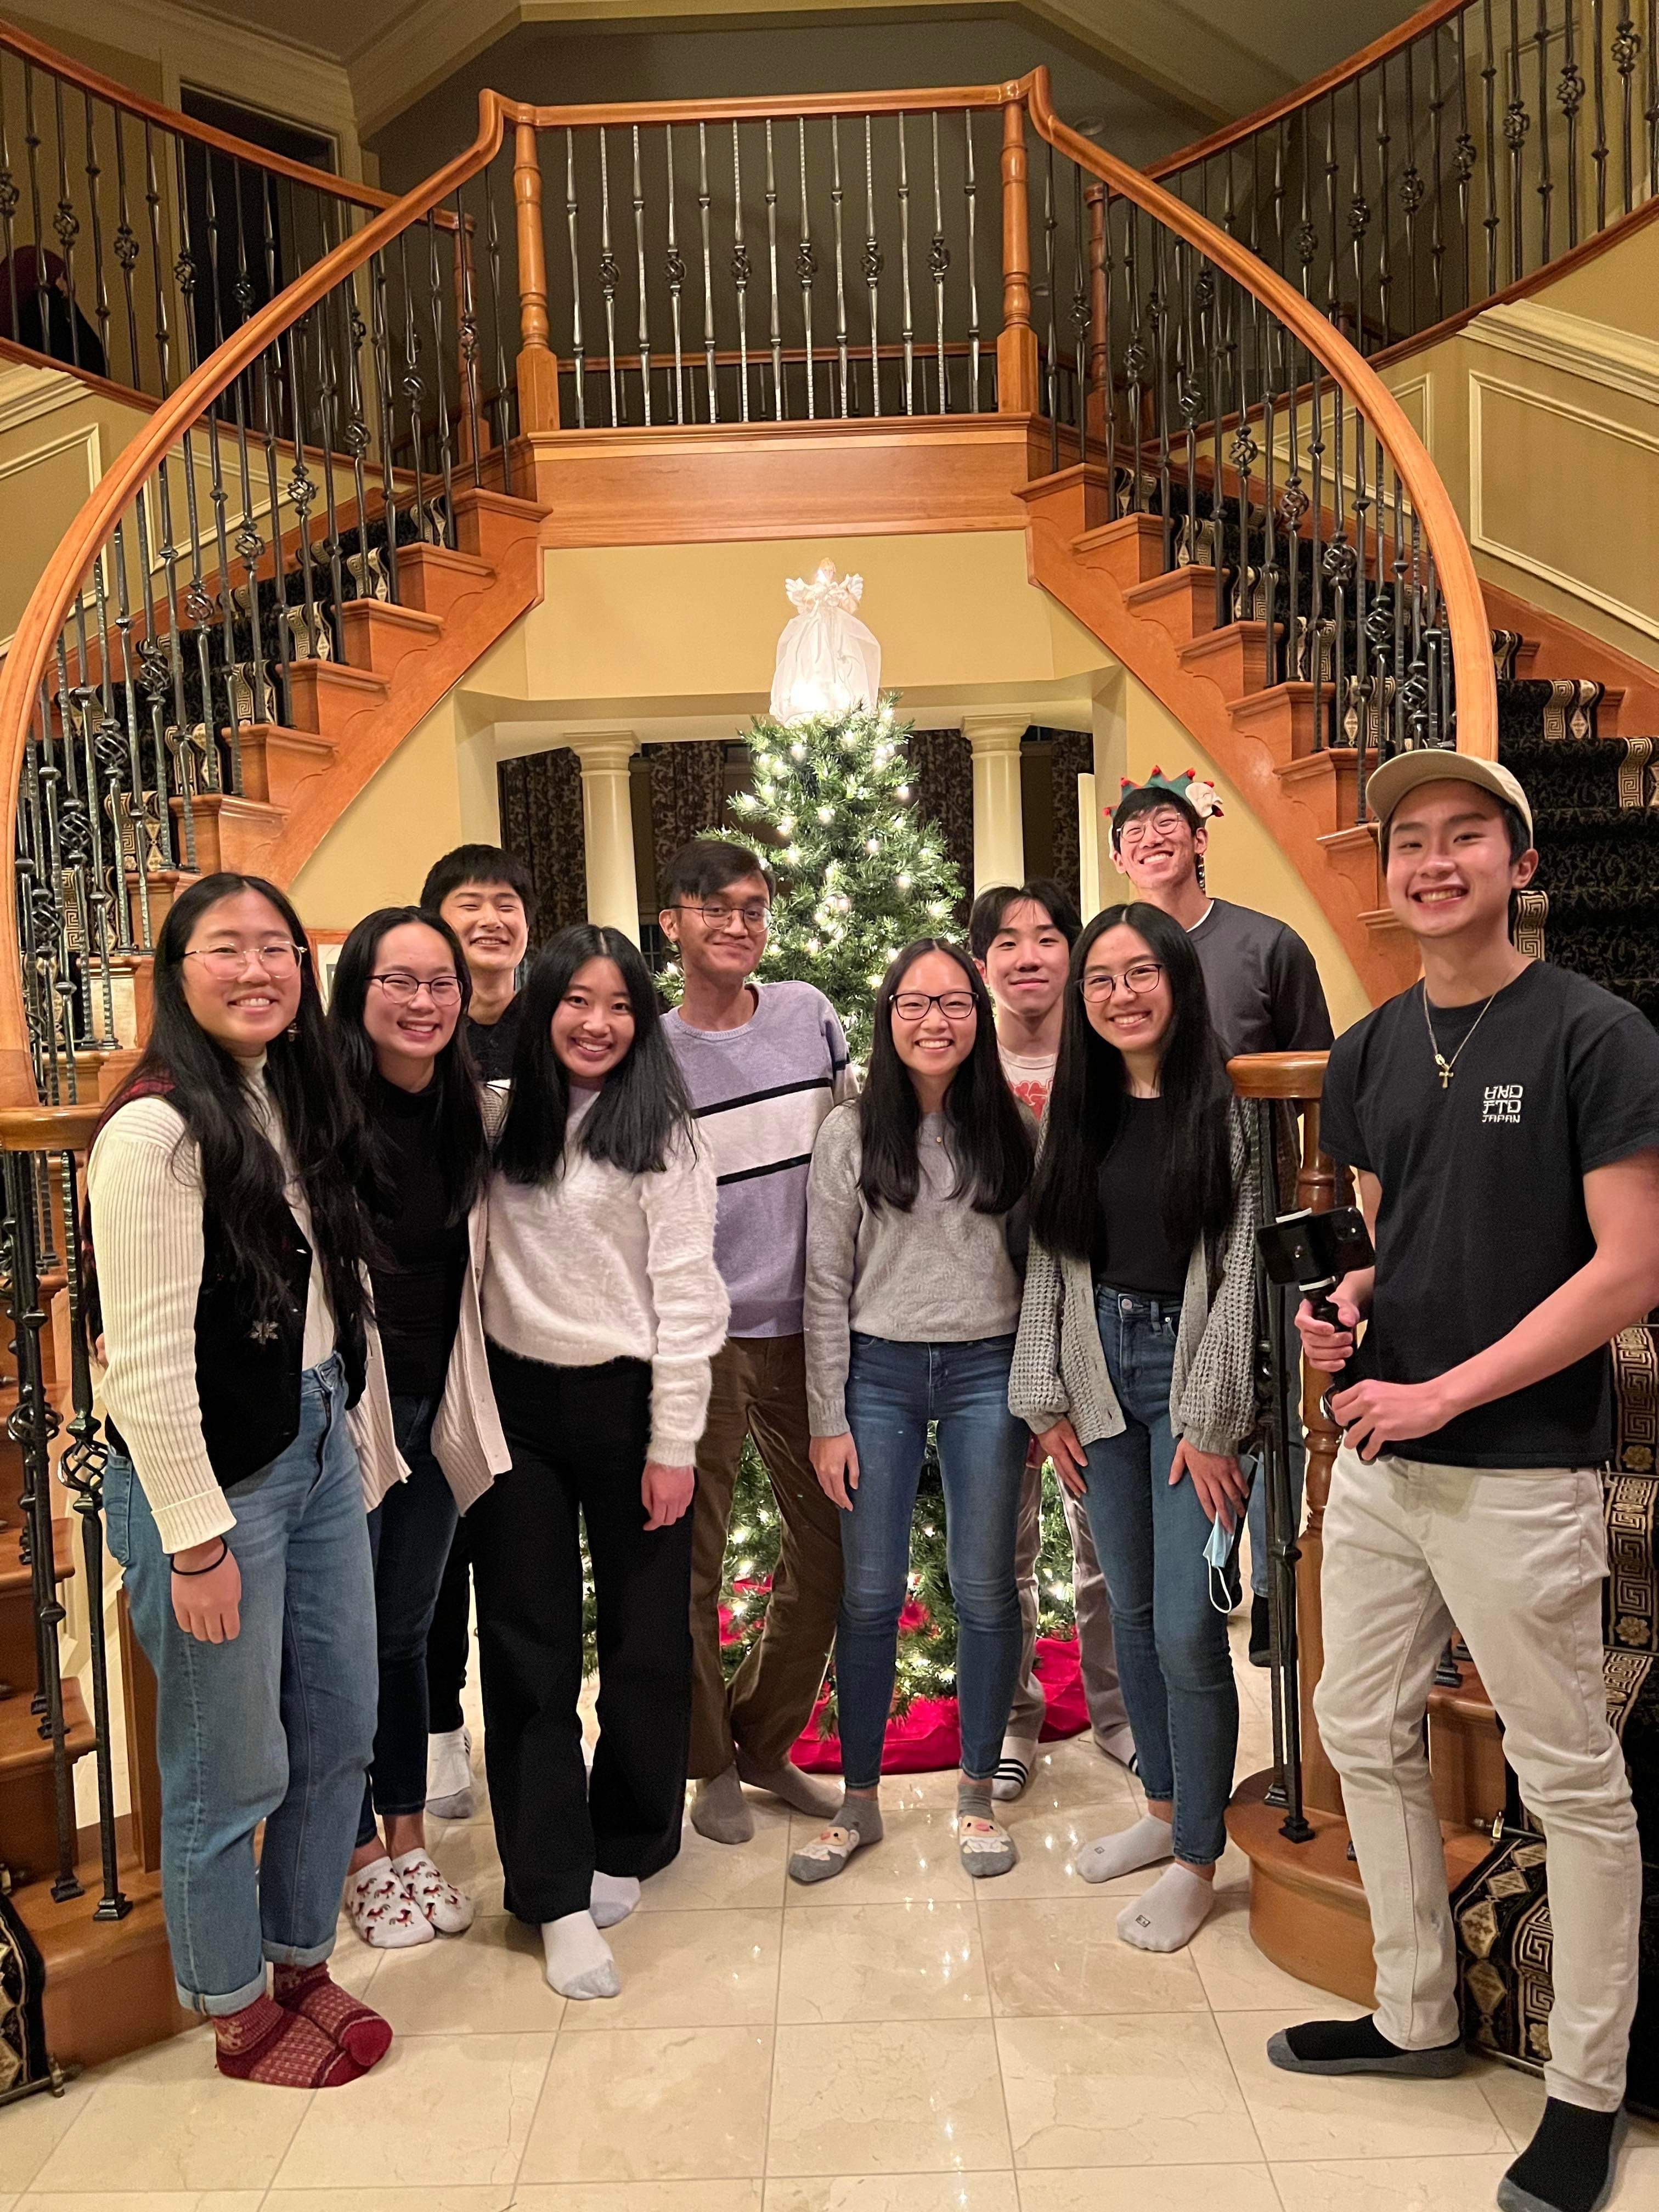
\includegraphics[width=0.25\textwidth,height=\textheight]{christmas.JPG}

\hypertarget{jalal-mawri}{%
\section{Jalal Mawri}\label{jalal-mawri}}

Current Master of Business Analytics student at the Ross School of Business

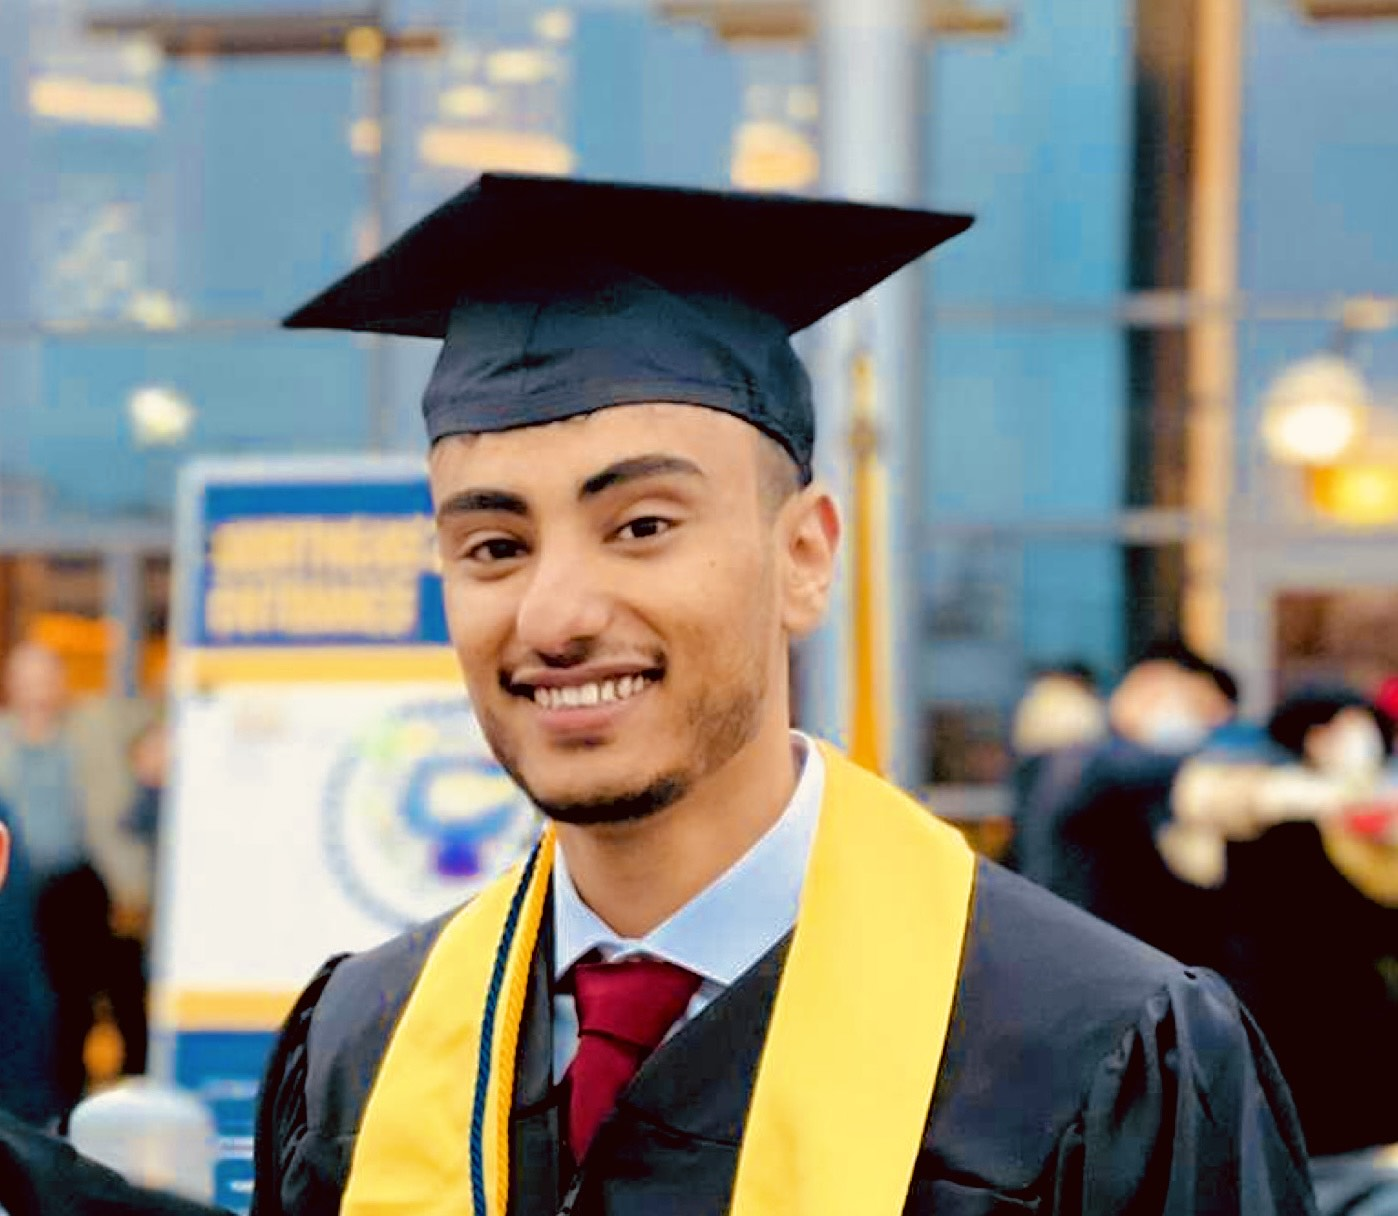
\includegraphics[width=0.25\textwidth,height=\textheight]{jalal1.jpg}
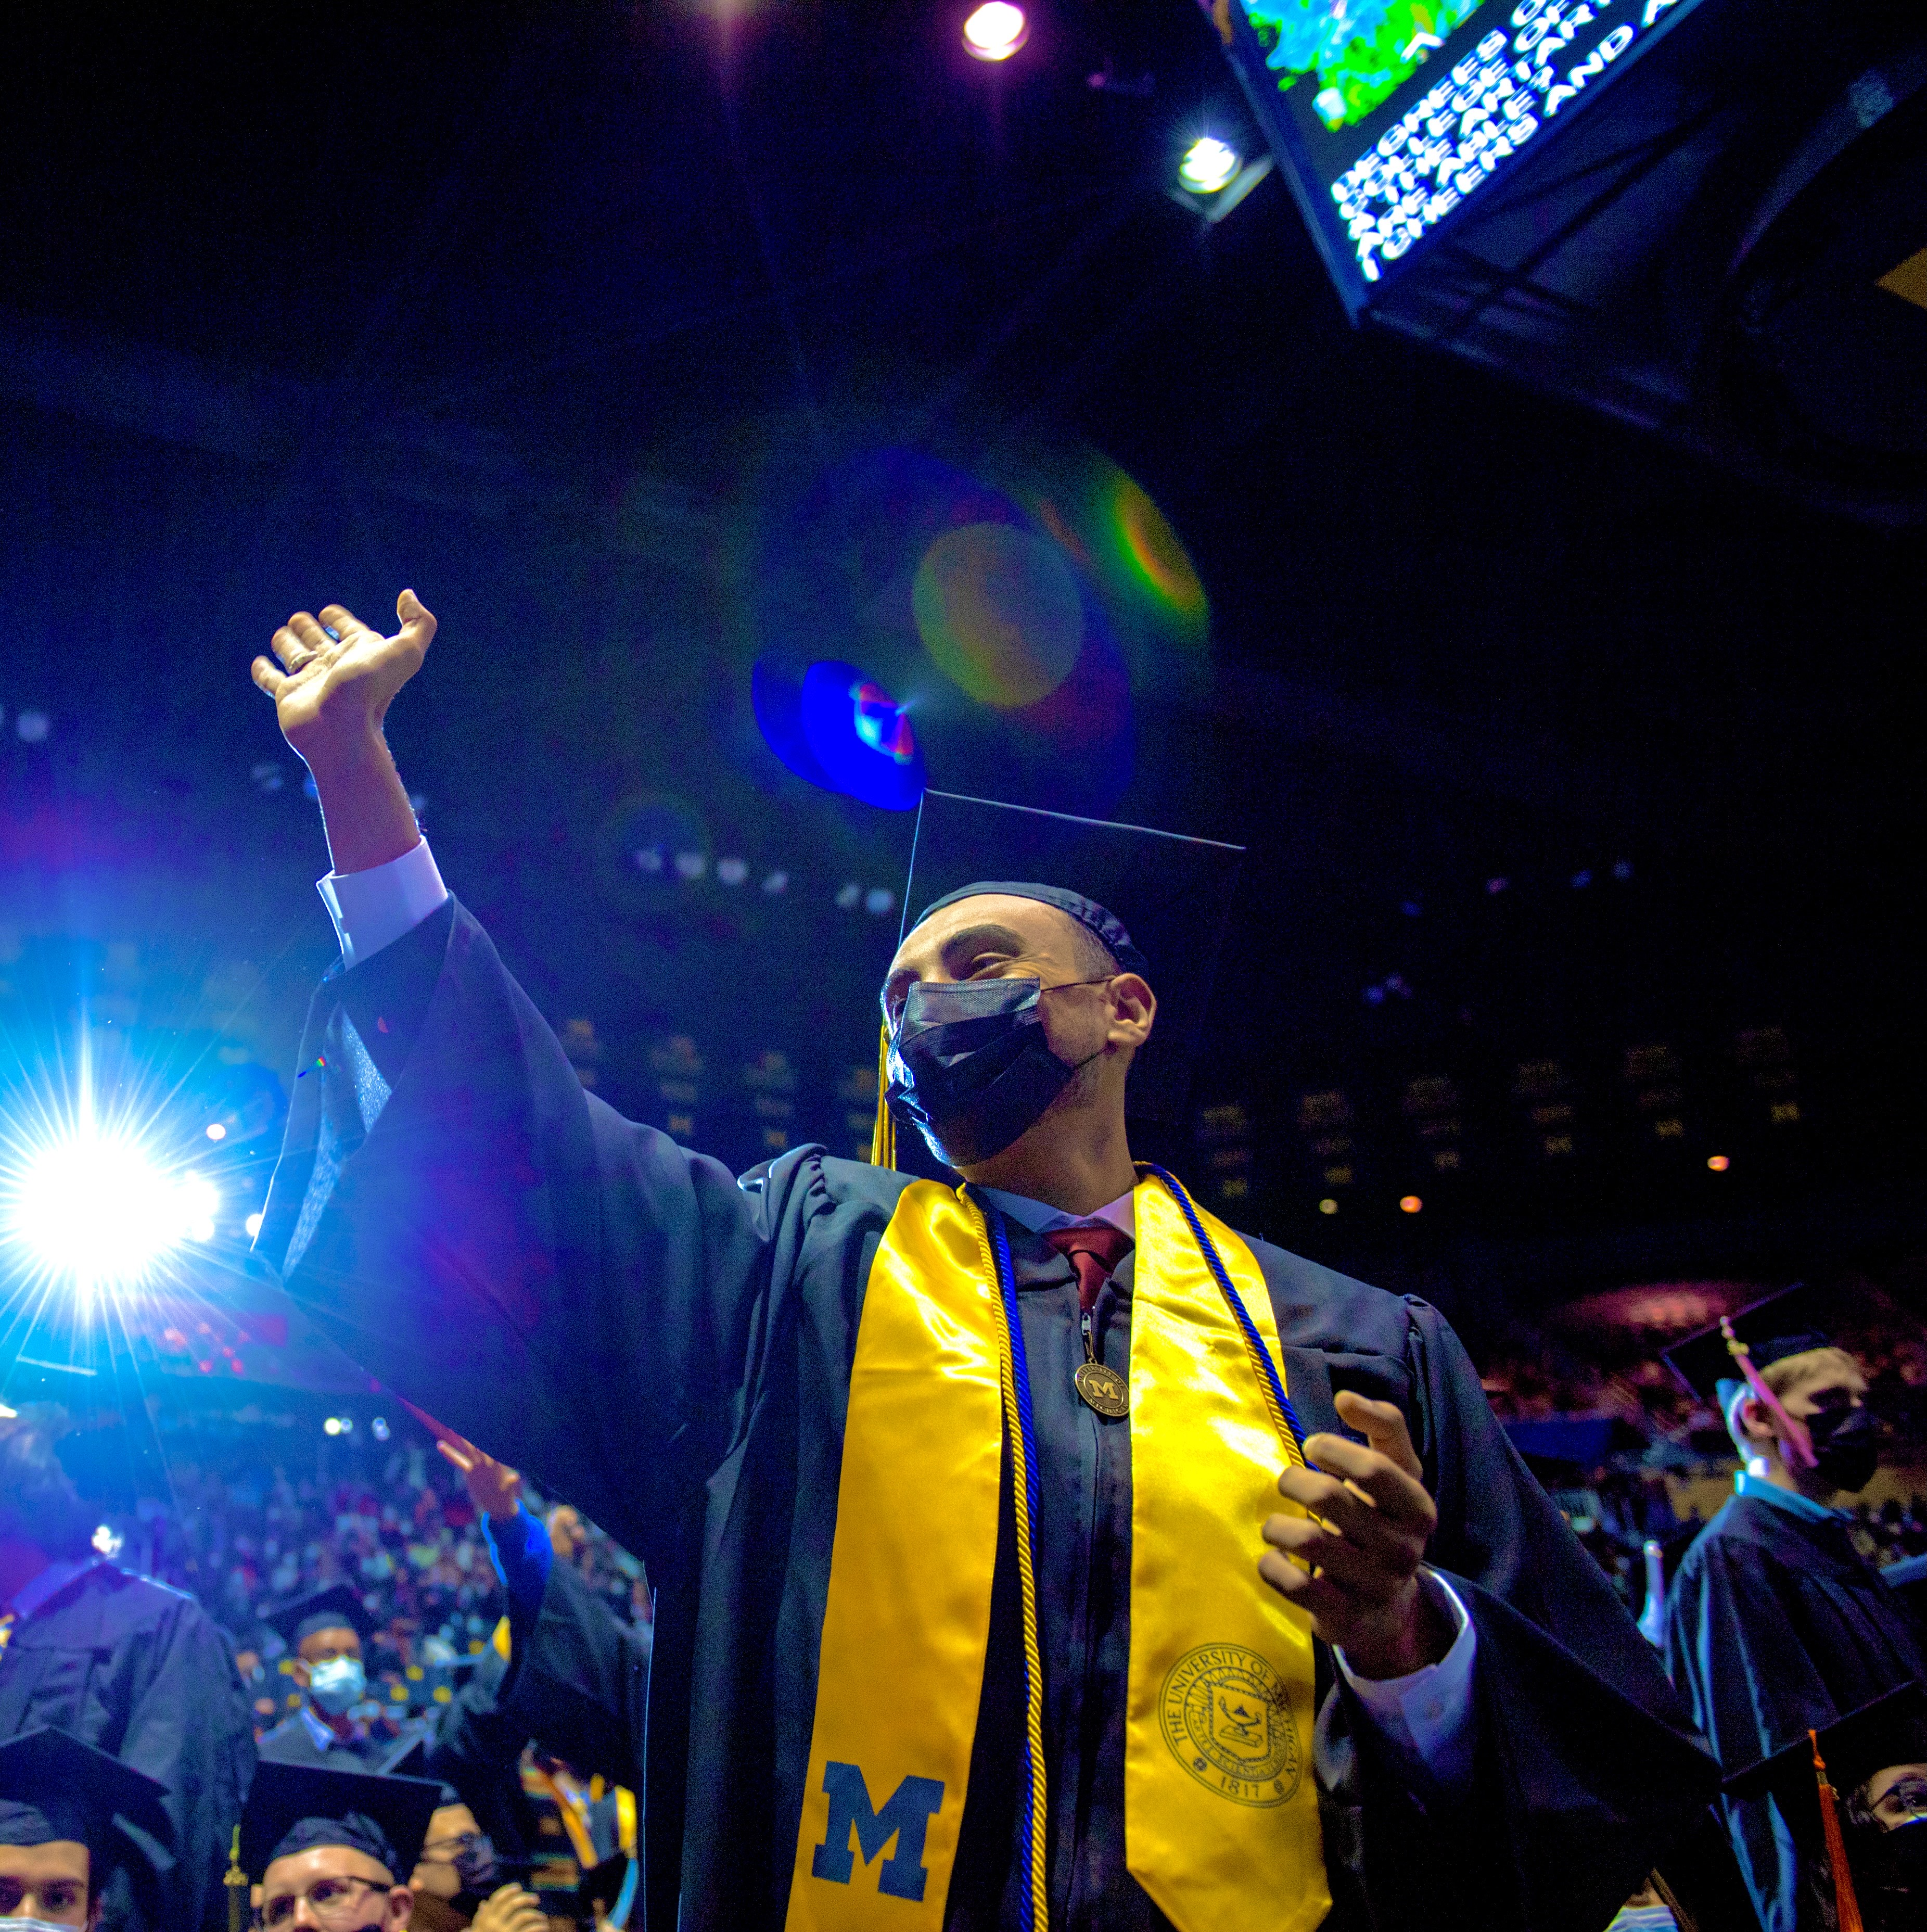
\includegraphics[width=0.25\textwidth,height=\textheight]{jalal2.jpg}
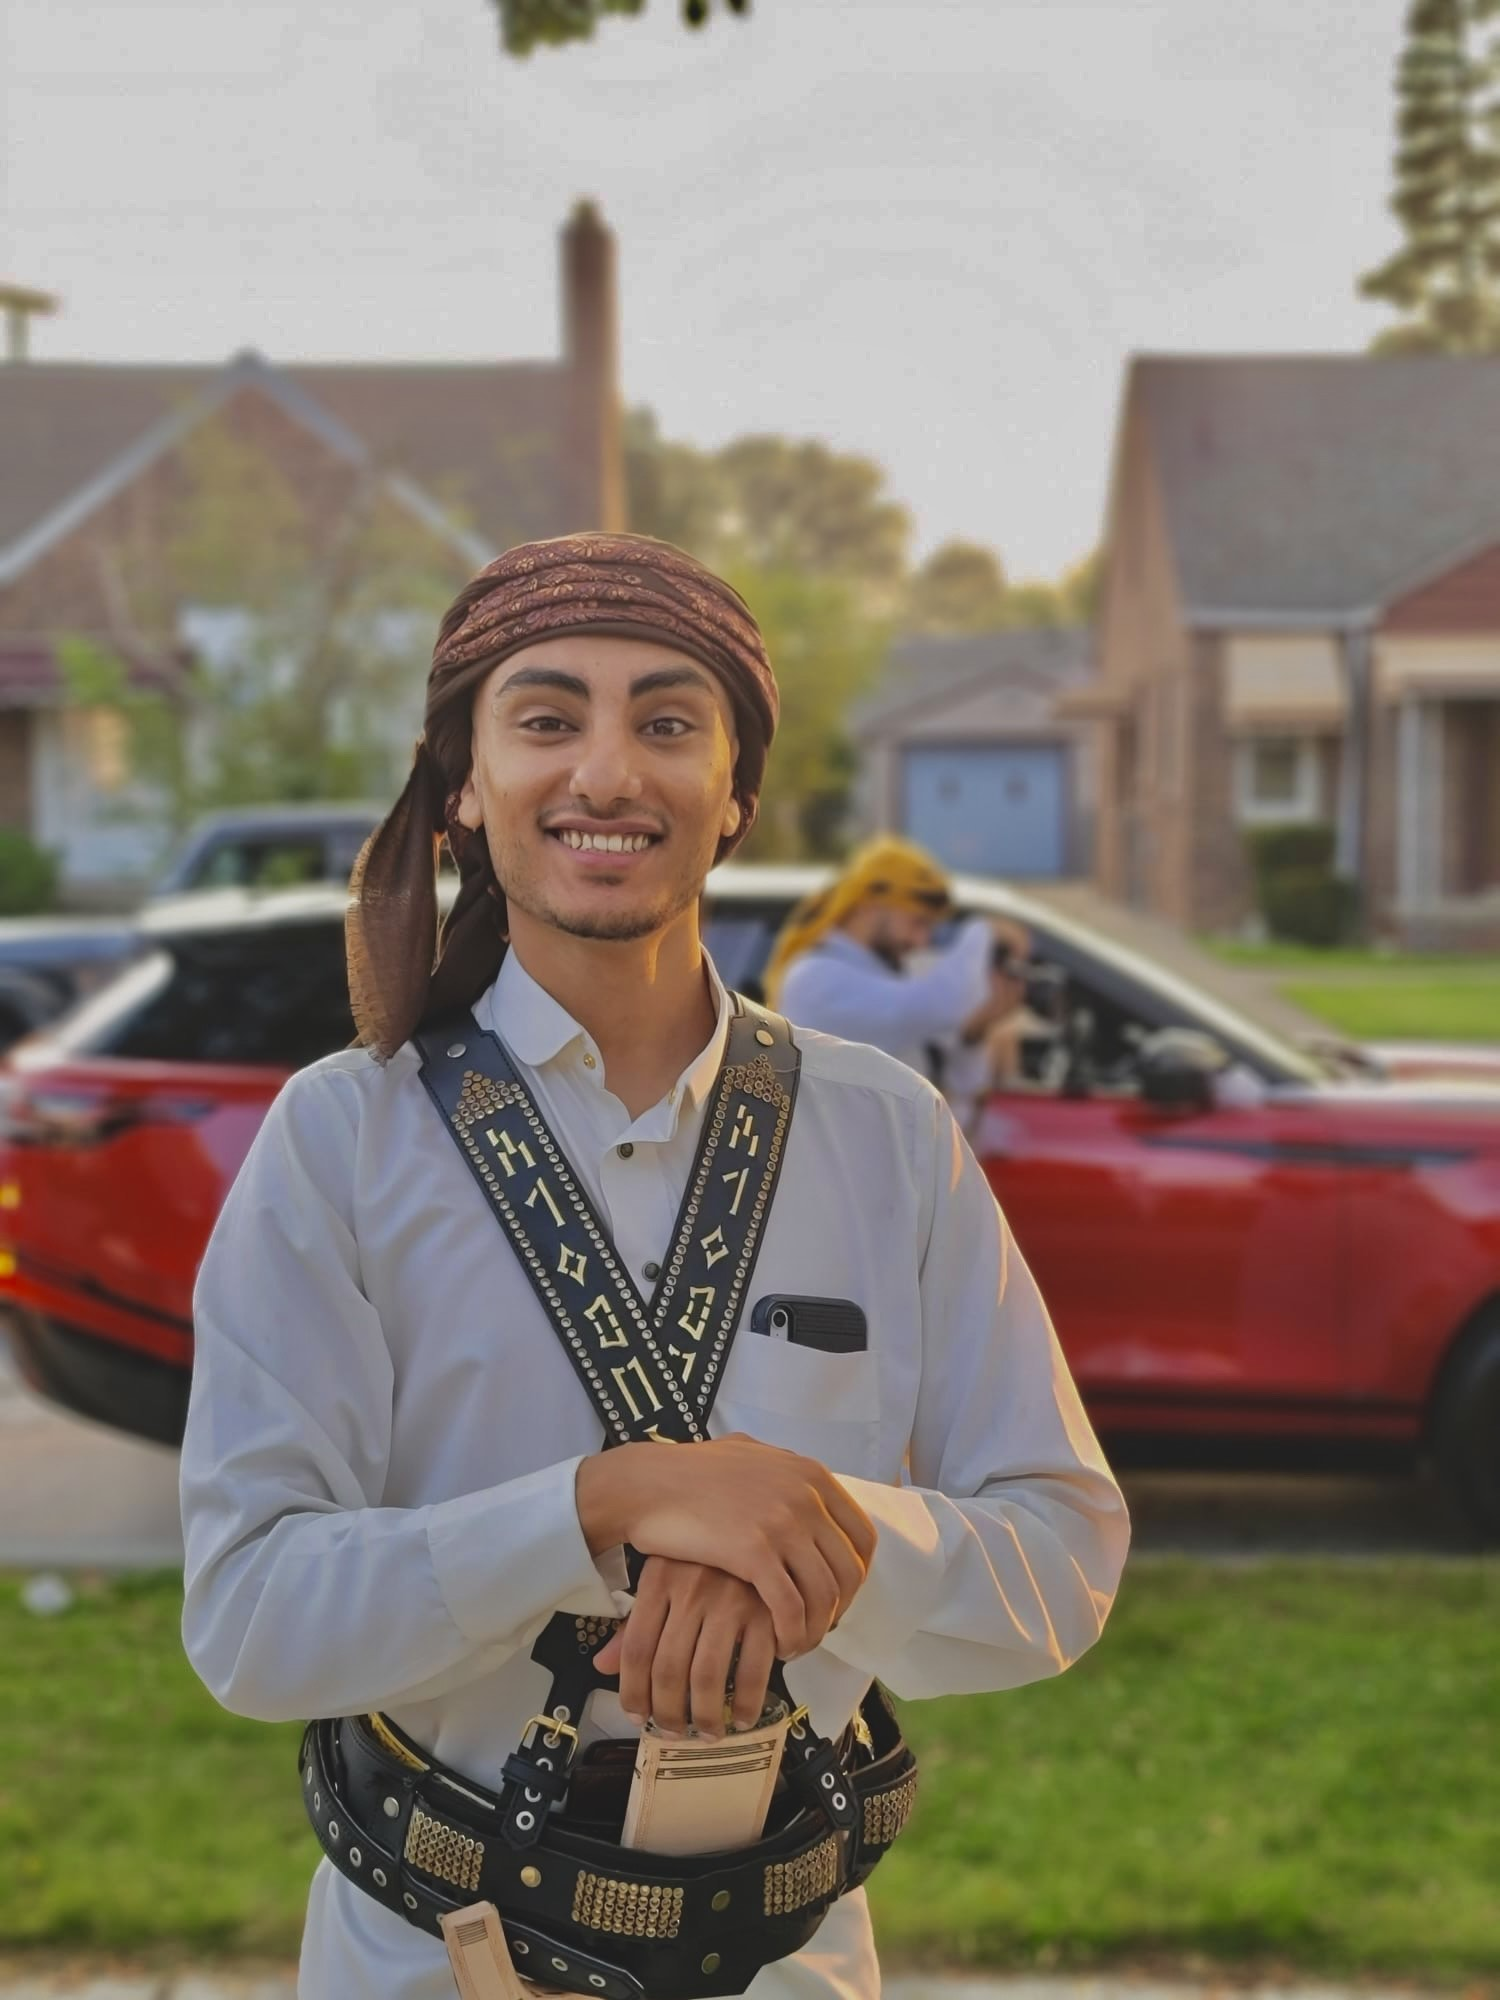
\includegraphics[width=0.25\textwidth,height=\textheight]{jalal3.jpg}

\textbf{Background}

I was born and raised in Yemen, the old city of Sana'a, and I left the country in 2013 with my family and immigrated to the United States. I grew up playing Football, a.k.a soccer, and my favorite team was and still is Manchester United.

\textbf{Education}

\begin{itemize}
\tightlist
\item
  I graduated from the University of Michigan with High Honors in Biology and International Studies.
\item
  During my first two years as an undergraduate student I had the opportunity to work on a research project at the Medical School where we researched preventive medical treatments for strokes.
\item
  During my senior year I wrote my thesis on the current civil war in Yemen, and I researched the Islamic Movement of Ansar Allah which is currently leading the political scene in Yemen and the Arabian Peninsula.
\end{itemize}

\textbf{Professional Experience}

\begin{itemize}
\tightlist
\item
  After graduating I interned for the Muslim Public Affairs Council, and worked on a project that persuaded the Biden Administration to enforce the reopening of Sana's Airport and push for a peace resolution between the parties involved in the war.
\item
  After my internship, I started to work as a Data Analyst for Amazon.
\item
  My plan after I graduate from Ross is to go back to Amazon and work as Business Intelligence Engineer.
\end{itemize}

\textbf{Publications}

Mawri, Jalal. ``Ansar Allah in Yemen: History and Ideology.'' Deep Blue Repositories, 1 Aug.~2021, \url{https://deepblue.lib.umich.edu/handle/2027.42/169403}.

Venugopal J, Wang J, Mawri J, Guo C, Eitzman D. Interleukin-1 receptor inhibition reduces stroke size in a murine model of sickle cell disease. Haematologica. 2021 Sep 1;106(9):2469-2477. doi: 10.3324/haematol.2020.252395. PMID: 32817286; PMCID: PMC8409048.

\hypertarget{housing}{%
\chapter{Housing}\label{housing}}

\hypertarget{finding-a-sublease}{%
\section{Finding a sublease}\label{finding-a-sublease}}

\textbf{Facebook groups -}
You can use these groups to find subleases to your liking. The posts usually specify the number of beds/baths, amenities, prices, pictures and contact info. Make sure to reach out to the subleaser through messenger. You can always negotiate and reduce the price as it is a buyers market in Ann Arbor.

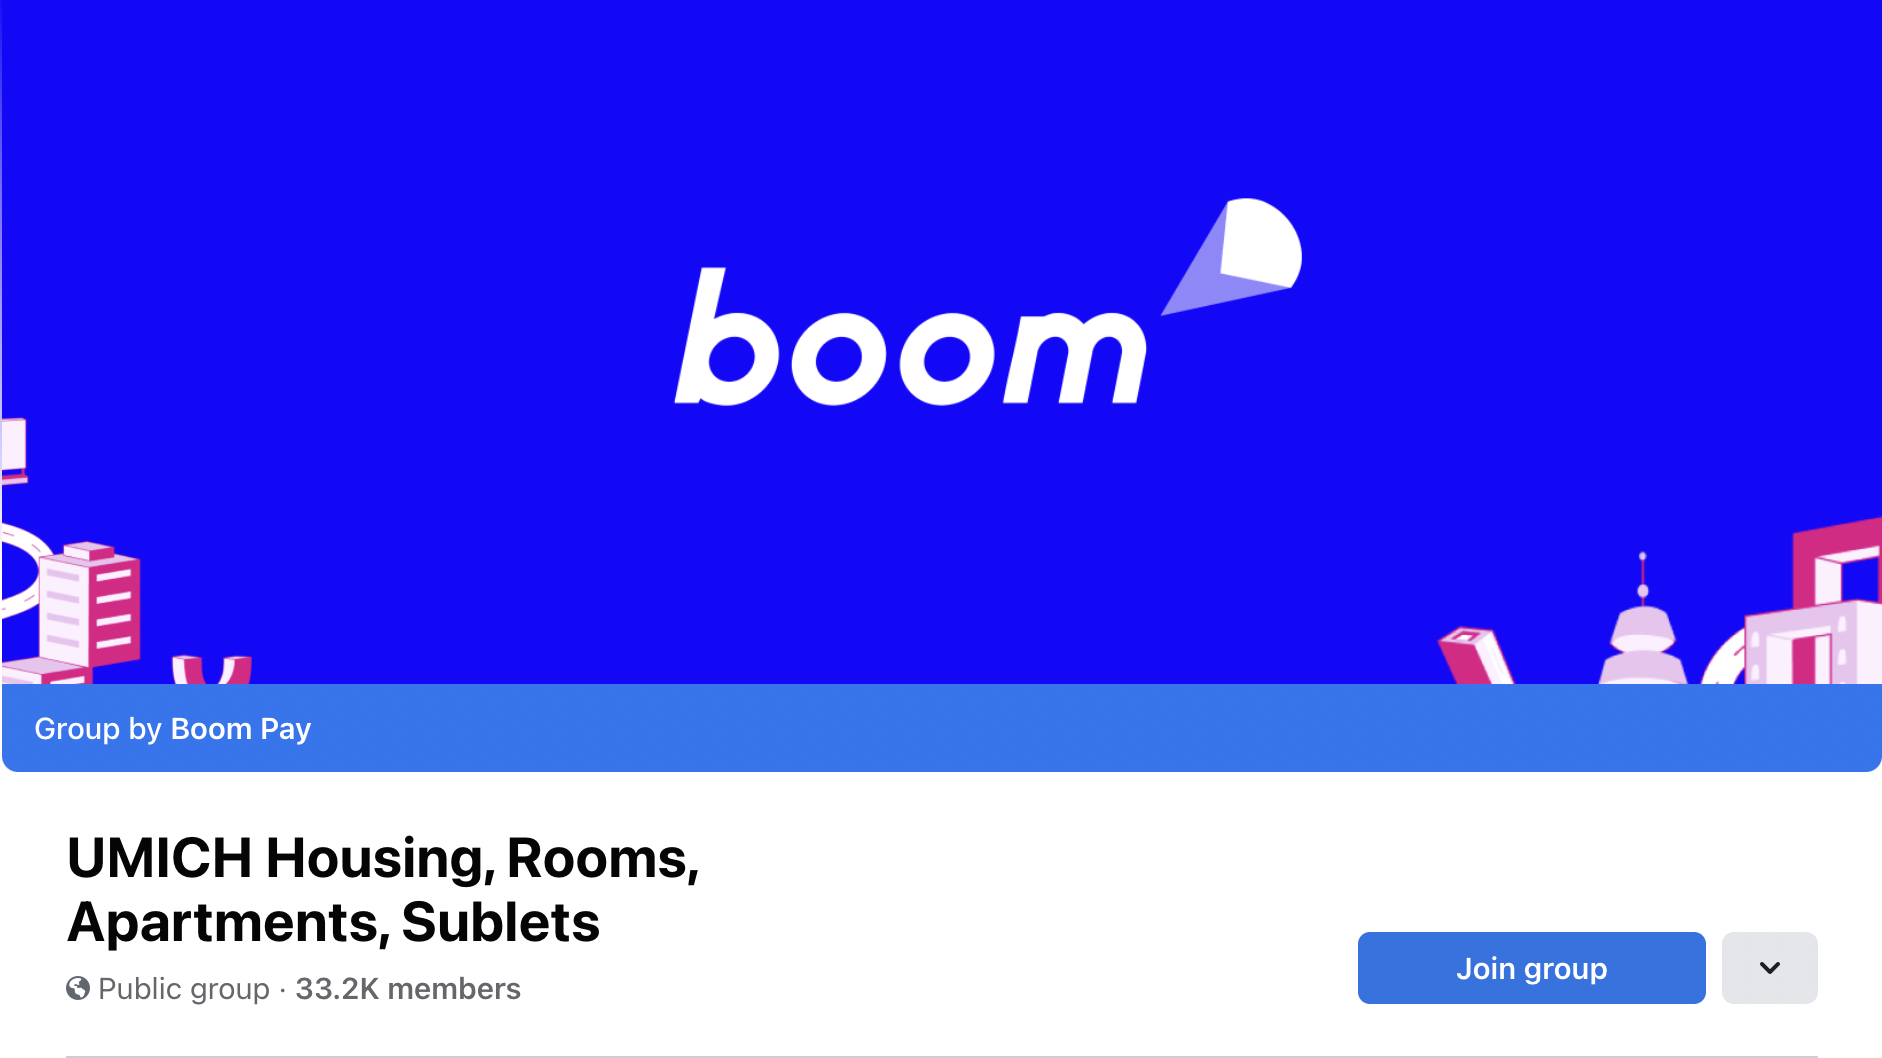
\includegraphics[width=3.125in,height=2.60417in]{Screen Shot 2022-08-03 at 3.05.44 PM.png}

\includegraphics[width=3.125in,height=2.60417in]{Screen Shot 2022-08-03 at 3.05.55 PM.png}
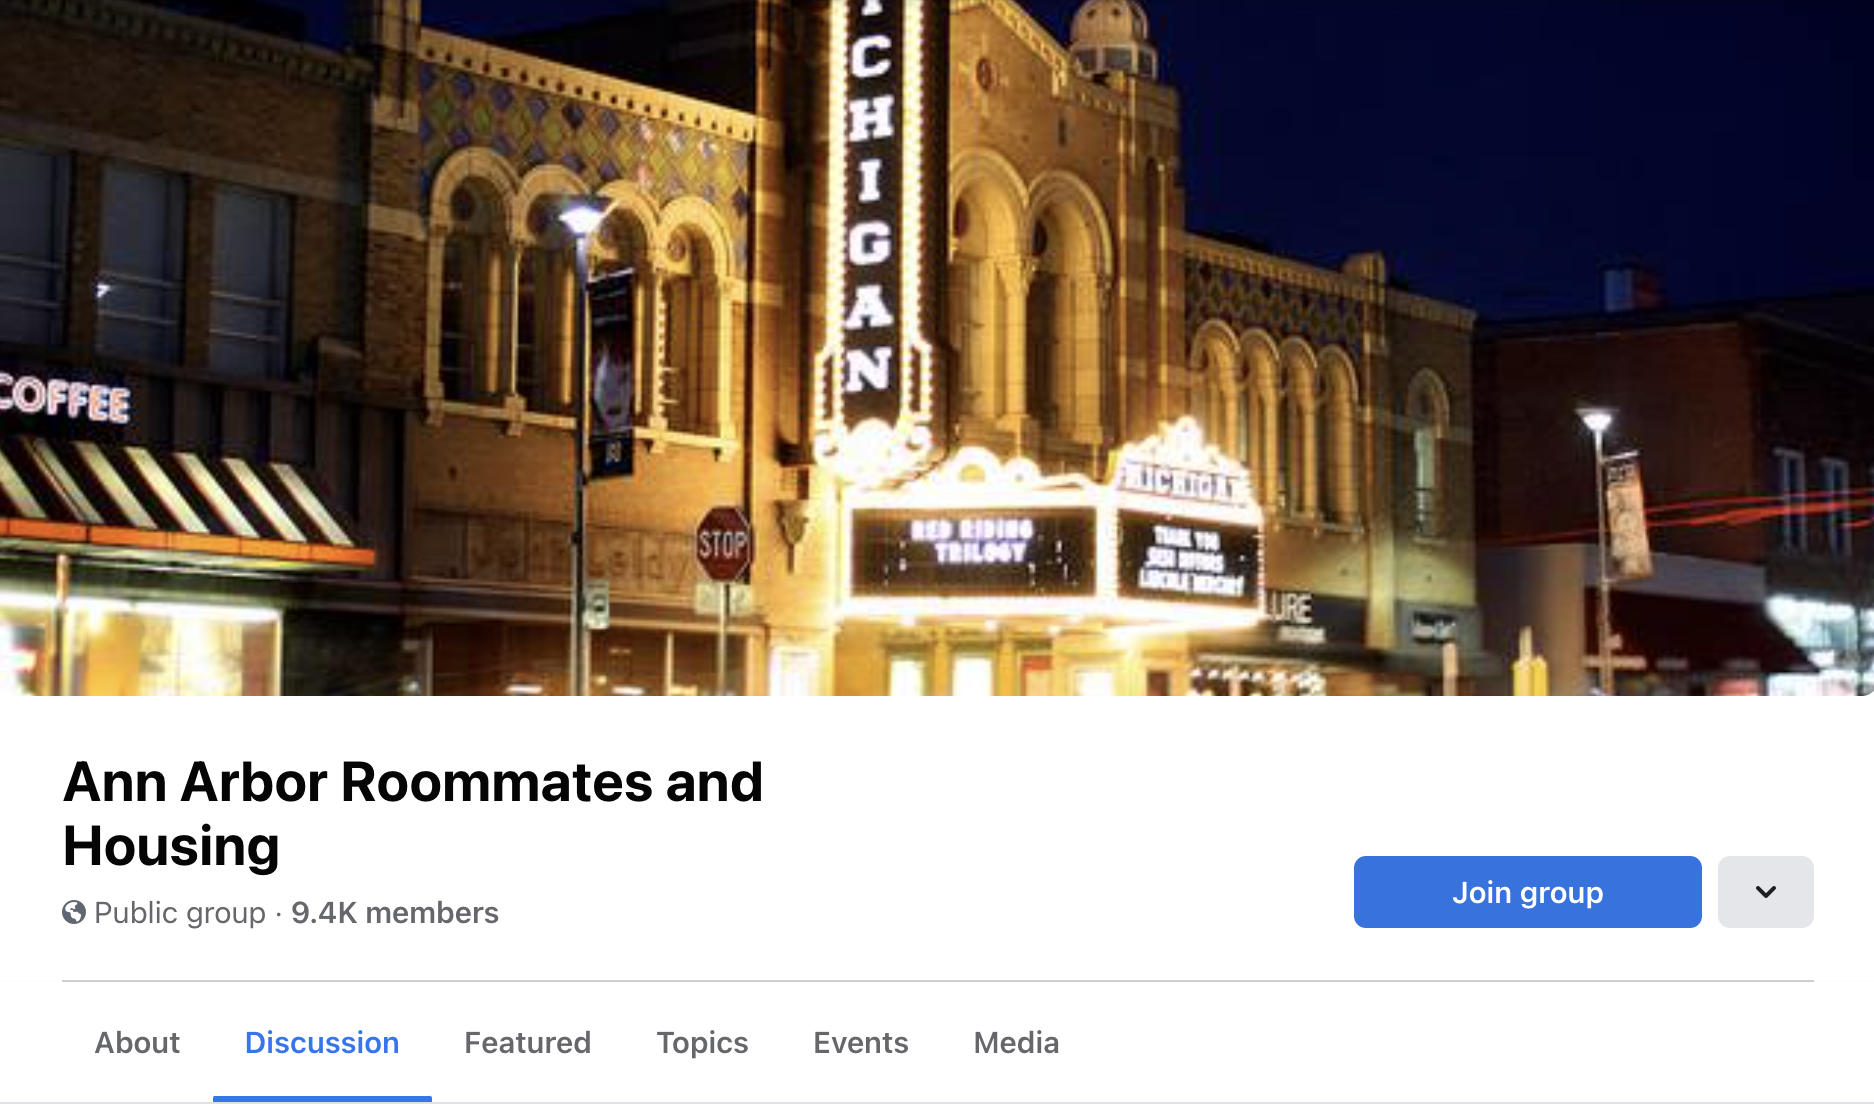
\includegraphics[width=3.125in,height=2.60417in]{Screen Shot 2022-08-03 at 3.06.08 PM.png}

\begin{itemize}
\tightlist
\item
  UMICH Housing, Rooms, Apartments, Sublets - (largest group with 33.4 K members)
  \url{https://www.facebook.com/groups/223351171575348/}
\item
  UMich Campus Housing (OFFICIAL)
  \url{https://www.facebook.com/groups/551056069413485/}
\item
  Ann Arbor Roommates and Housing
  \url{https://www.facebook.com/groups/267575123414633/}
\end{itemize}

\textbf{Pro Tips} - Have a video call with the subleaser and see the apartment for yourself if you are unable to visit, read google reviews and talk to current students to get a better idea of the apartment(location, management, maintenance)

\textbf{Calling Apartments: }
Another method that works would be to call the different apartments in areas you are interested in and ask them if any residents are interested in subleasing. They will connect you with subleasers or add you to their addressbook so they can reach out anytime any sublease becomes available.

You could also ask for a lease transfer though this is a more expensive option as you need to pay the entire rent for the month. Lease transfers/takeovers are more useful if you want the lease for the entire academic year.

\textbf{WeChat - }
UM信息平台
Wechat number: UMhome
You can use this user id from WeChat to find available sublets by accessing the moments page.

\hypertarget{lease-subletting-information}{%
\section{Lease Subletting Information}\label{lease-subletting-information}}

\hypertarget{who-this-page-is-for}{%
\subsection{Who this page is for:}\label{who-this-page-is-for}}

\begin{itemize}
\tightlist
\item
  Current MBAn students wishing to sublet their current leases to future MBAn studets
\item
  Prospective and admitted MBAn students wanting to find housing for the former or latter part of their experience
\end{itemize}

\hypertarget{you-want-to-sublet-your-lease}{%
\subsection{You Want to Sublet Your Lease}\label{you-want-to-sublet-your-lease}}

So, you want to sublet your lease, but have had trouble finding someone. Great! We have taken the pain out of this process by connecting you with future MBAn students hungry to find a place to stay for a few months before their lease starts. To get started, just fill out this form. Interested students will be able to see all of this information and will contact you if they are interested.

Form: \url{https://docs.google.com/forms/d/e/1FAIpQLSfd5a1n3rtsh2xlqPA1M3tiaQFIl-nXuANBcQ9awZvN5U2sag/viewform}

\hypertarget{you-need-a-place-to-stay}{%
\subsection{You Need a Place to Stay}\label{you-need-a-place-to-stay}}

Your lease doesn't start until August, so you need a place to stay for the summer. Or, your lease ends early and you need a place to stay for those last few month of the MBAn program. No problem! In the Google Sheet below, you will find a list of current MBAn students wishing to sublet their lease. Plenty of information about the properties is included in this document, but if you need more info, don't hesitate to reach out--contact information is provided. Happy shopping!

Sheet: \url{https://docs.google.com/spreadsheets/d/1nCS9Tw-RBSAceeZNXqH_YfsoTt1rkVl-x5Z3lqS9AoQ/edit?resourcekey\#gid=536291696}

\hypertarget{dorms}{%
\section{Dorms}\label{dorms}}

Graduate Residence Options for incoming MBAn students

Option 1: Munger Graduate Residence

Address: 540 Thompson St, Ann Arbor, MI 48104

Phone: 734-764-0145

E-mail: \href{mailto:msaraino@umich.edu}{\nolinkurl{msaraino@umich.edu}}

Price: \$1100/Month -\textgreater{} \$2000/Month

Description:
Located on Central Campus, the Munger Graduate Residences are designed specifically for graduate and professional level students from all U-M schools and colleges to actively engage in a transdisciplinary community. Transdisciplinary living brings a diverse mix of graduate and professional students from various fields together to live, study and build a culture of collaboration. You'll join other graduate students in a furnished apartment with 6 or 7 single-occupancy bedroom suites, each with a private bathroom. The suites also include a very large kitchen, dining room and community space.

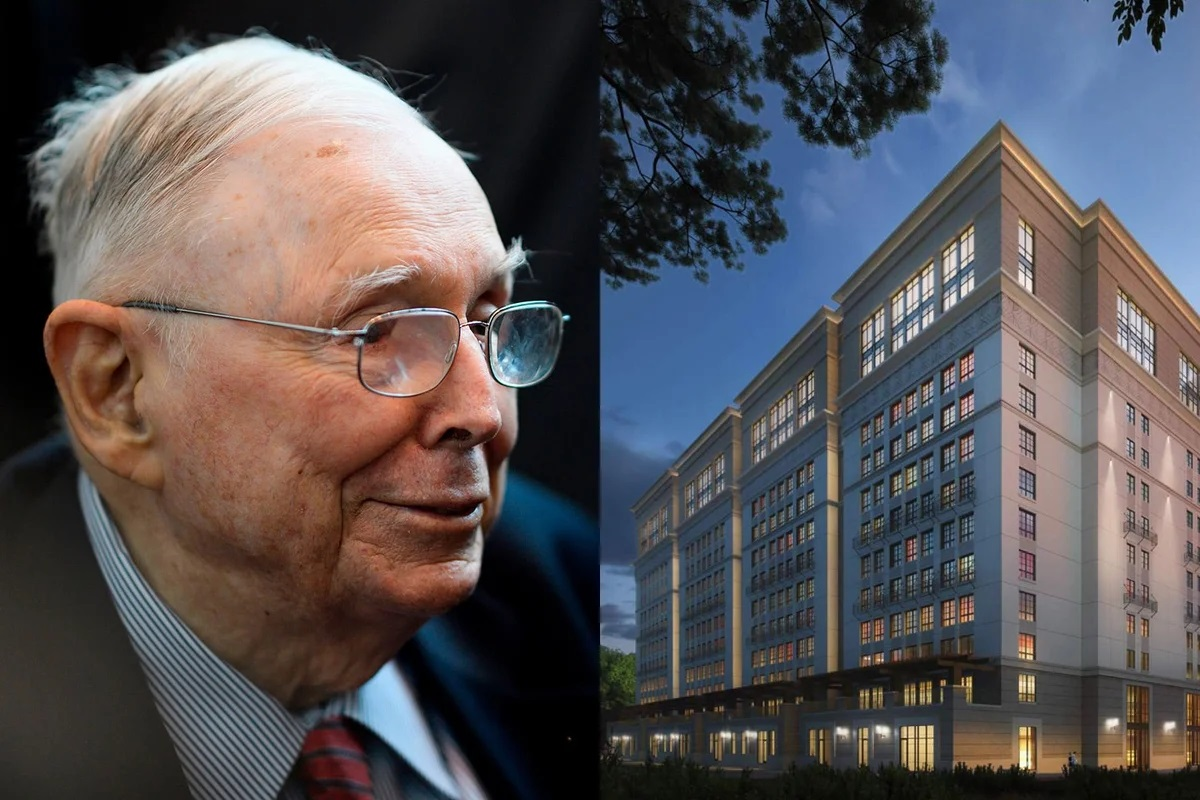
\includegraphics[width=2.66667in,height=\textheight]{MUNGER1.jpg}

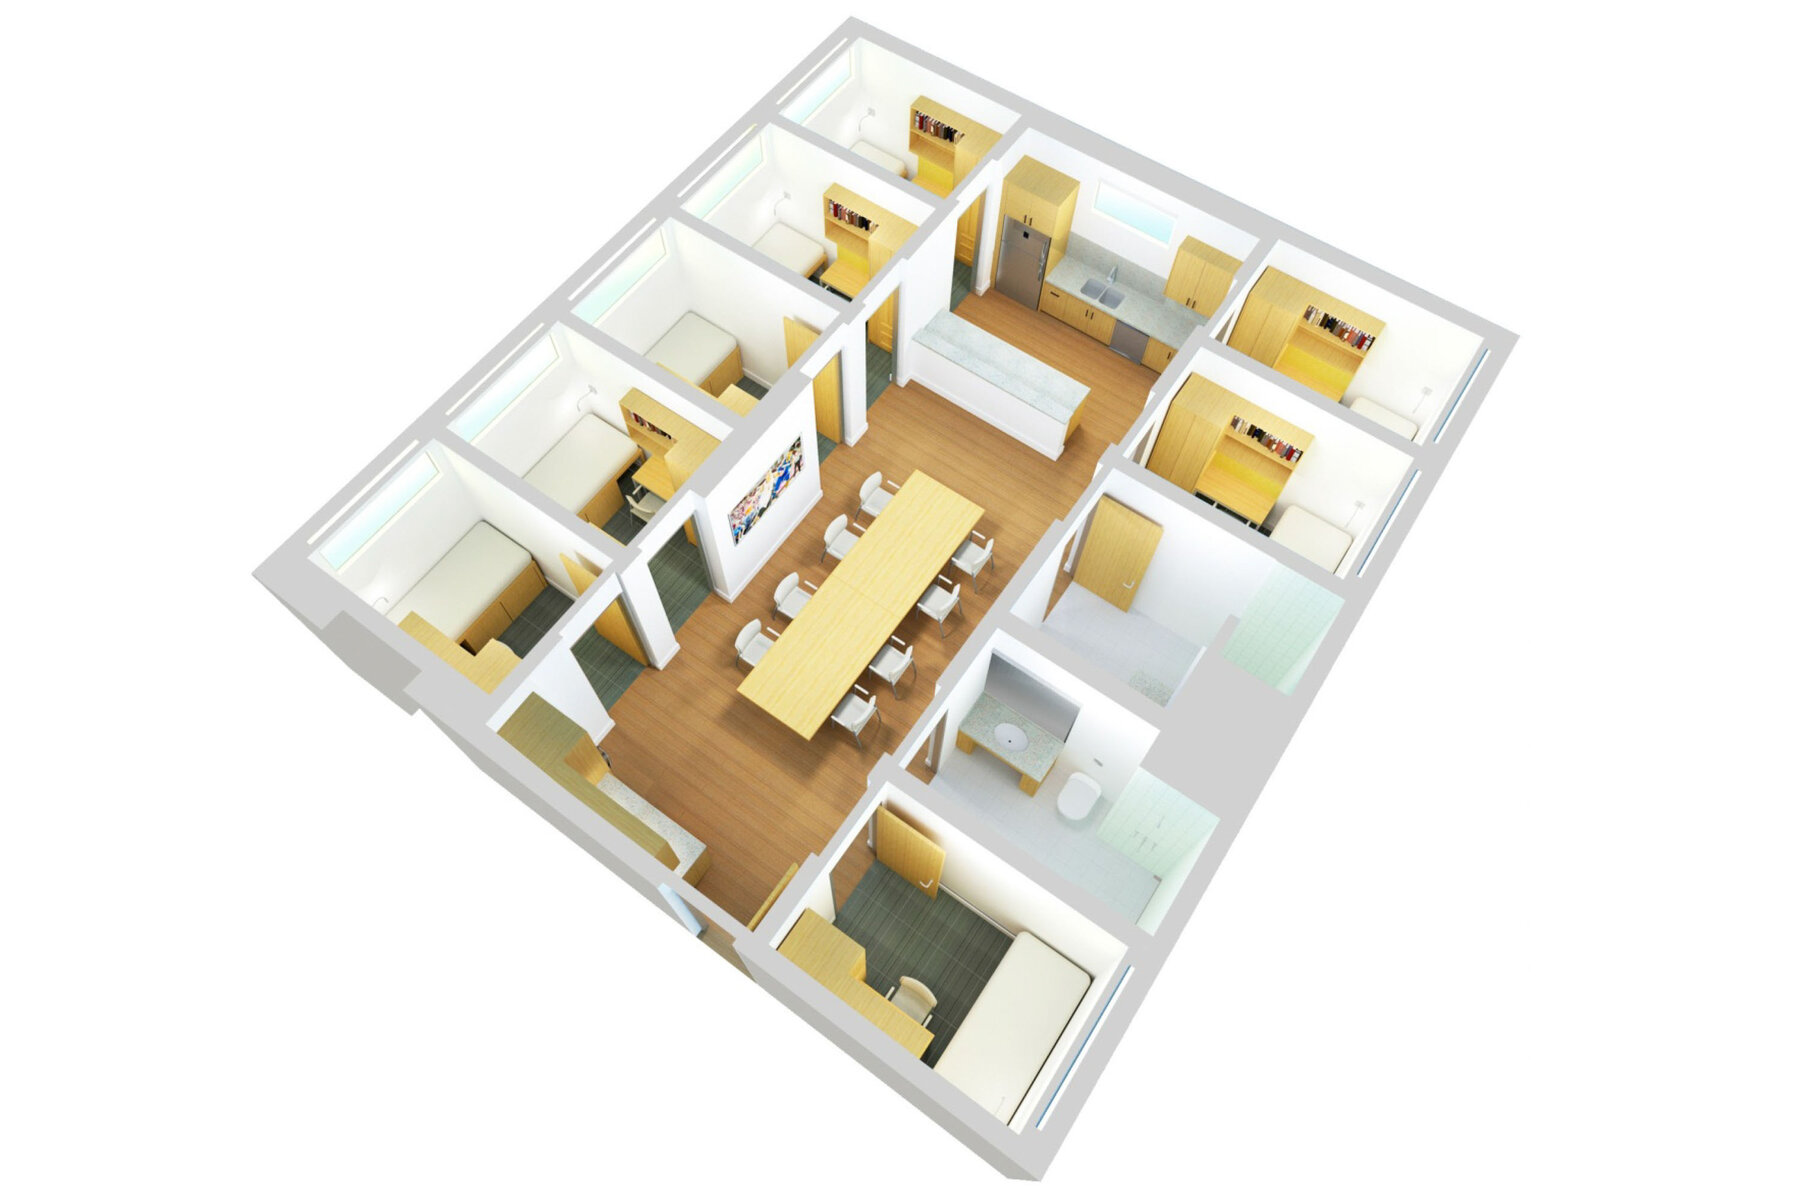
\includegraphics[width=2.66667in,height=\textheight]{MUNGER2.jpg}

Option 2: EAST QUADRANGLE

Address:701 East University Avenue, Ann Arbor, MI 48109-1245

Phone: 734-764-0100

E-mail: \href{mailto:msaraino@umich.edu}{\nolinkurl{msaraino@umich.edu}}

Price: \$1100/Month -\textgreater{} \$2000/Month

Description:
East Quad, a mixed-gender, undergraduate residence hall, is home to approximately 850 students each year. It's on Central Campus near the South University shopping area and many academic buildings including Ross School of Business and the School of Education.

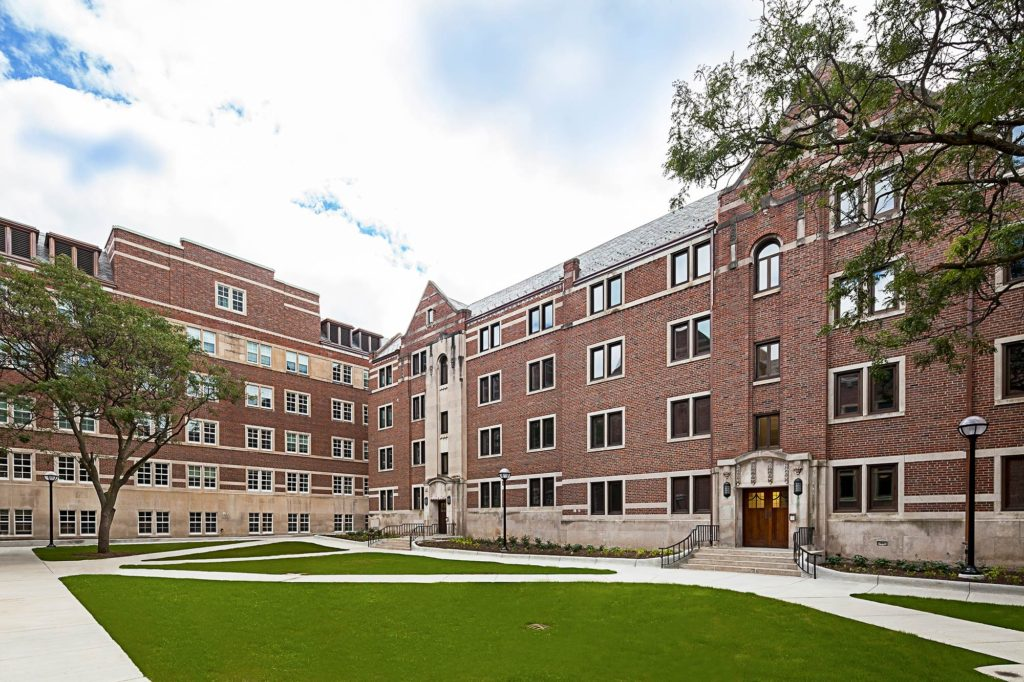
\includegraphics[width=2.66667in,height=\textheight]{EQUA2.jpg}

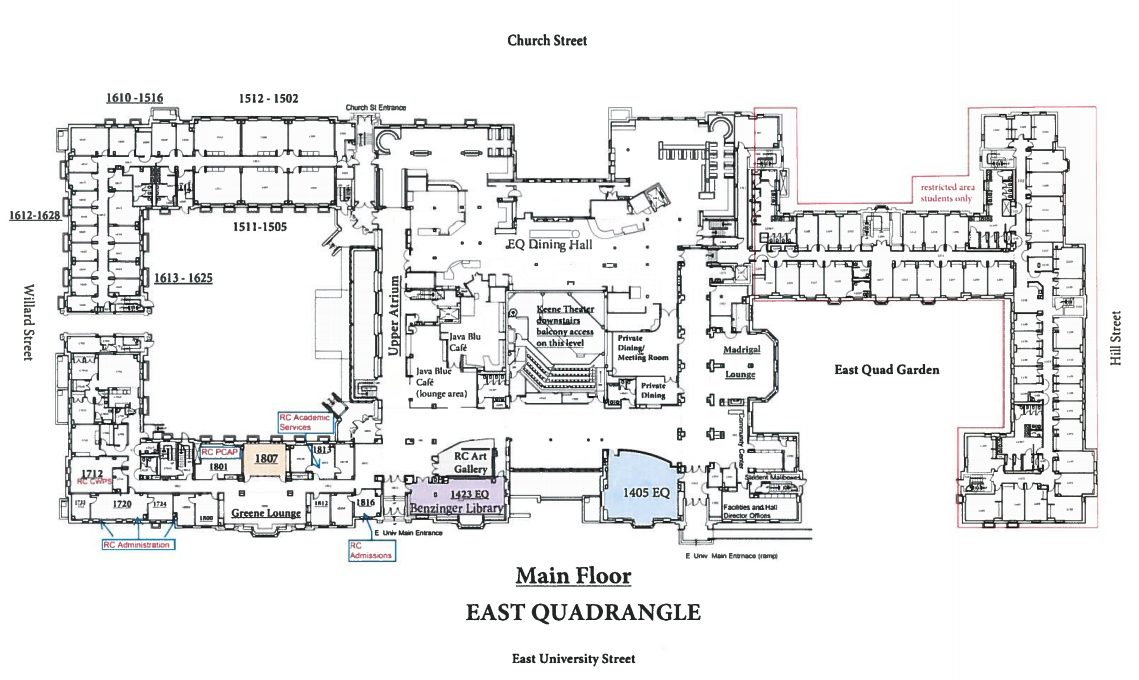
\includegraphics[width=2.66667in,height=\textheight]{EQUA1.jpg}

\hypertarget{high-rise-apartments}{%
\section{High-rise Apartments}\label{high-rise-apartments}}

\hypertarget{central-campus}{%
\subsection{Central Campus}\label{central-campus}}

\hypertarget{apartments-near-ross}{%
\subsection{Apartments Near Ross}\label{apartments-near-ross}}

\begin{itemize}
\tightlist
\item
  Foundry Lofts
\end{itemize}

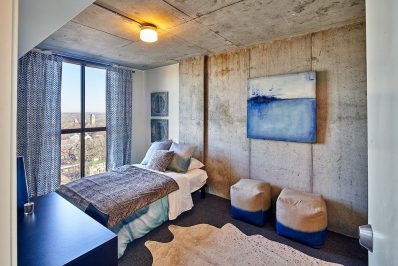
\includegraphics[width=0.32\textwidth,height=\textheight]{Foundry_Lofts_inside_1.jpg}
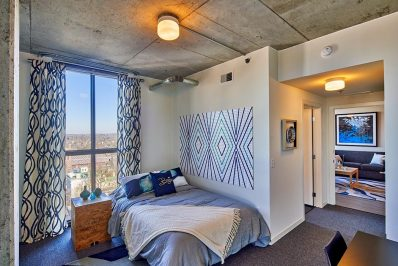
\includegraphics[width=0.32\textwidth,height=\textheight]{Foundry_Lofts_inside_2.jpg}
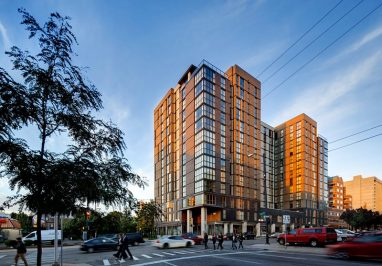
\includegraphics[width=0.31\textwidth,height=\textheight]{Foundry_Lofts_outside_1.jpg}

\begin{center}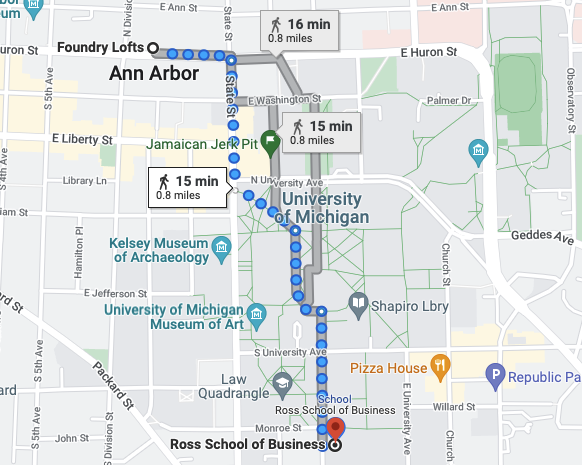
\includegraphics{Foundry map} \end{center}

\textbf{Website:} \url{https://www.foundryloftsannarbor.com/?utm_medium=market_site\&utm_campaign=market_site\&utm_source=liveumich}

\textbf{Floor plans:}
Studio, 1-, 2-, 3-, \& 4-Bedroom Apartments

\textbf{Description:}
If you're looking for a lavish living experience with exclusive amenities, a premier location just minutes from campus, and the latest in interior apartment features, Foundry Lofts is right for you. Enjoy scenic views from the rooftop deck, stay productive in the work and study lounge, or satisfy late-night cravings at our ground-floor retail area. With fully furnished floor plans featuring private bedrooms and bath suites, expansive closets, stainless steel appliances, and so much more, Foundry Lofts offers everything one needs to live in style and comfort. With the needs of young professionals in mind, Foundry Lofts seamlessly weaves features to promote academics and socialization with a community that feels like home.

\textbf{Pros:}
Near Local Restaurants \& Retail in Downtown

\begin{itemize}
\tightlist
\item
  Saga Ann Arbor
\end{itemize}

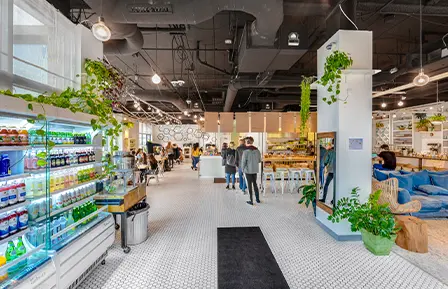
\includegraphics[width=0.32\textwidth,height=\textheight]{saga interior.jpg}
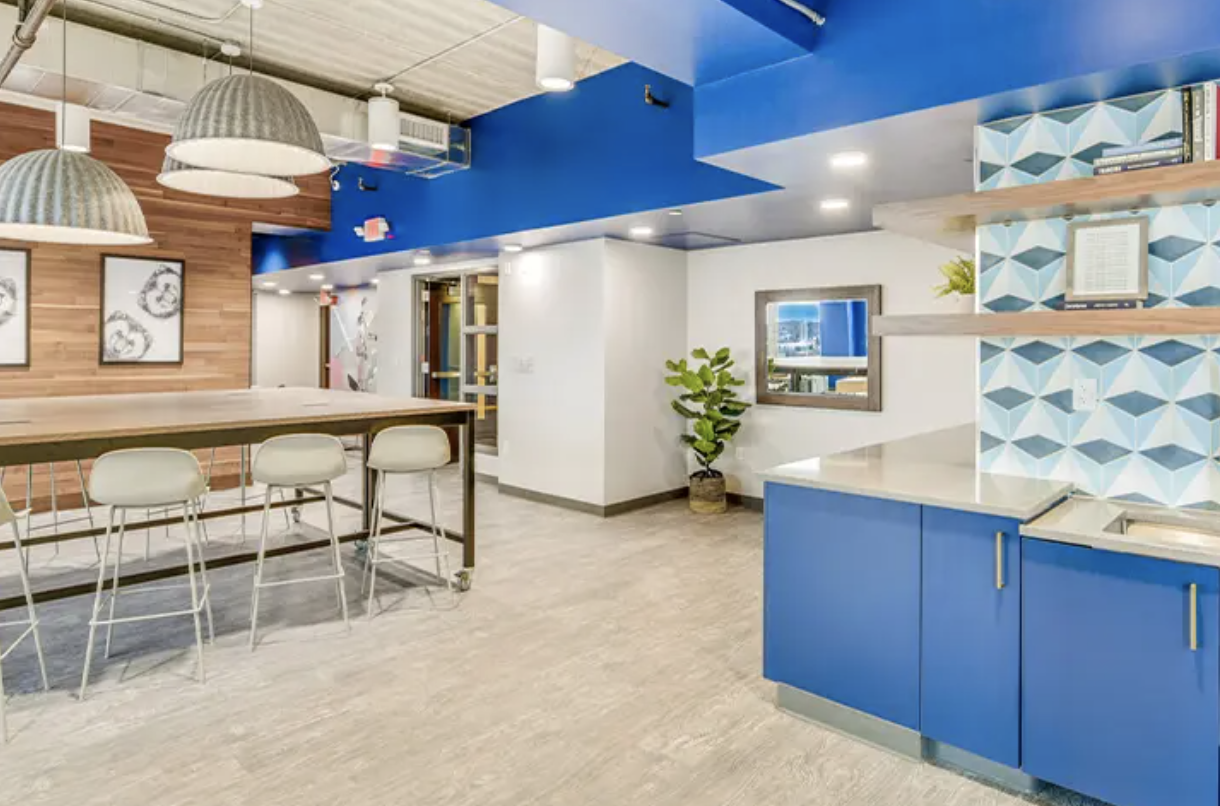
\includegraphics[width=0.32\textwidth,height=\textheight]{saga interior 2.jpg}
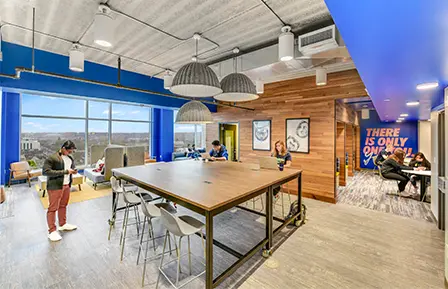
\includegraphics[width=0.31\textwidth,height=\textheight]{saga interior 3.jpg}

\begin{center}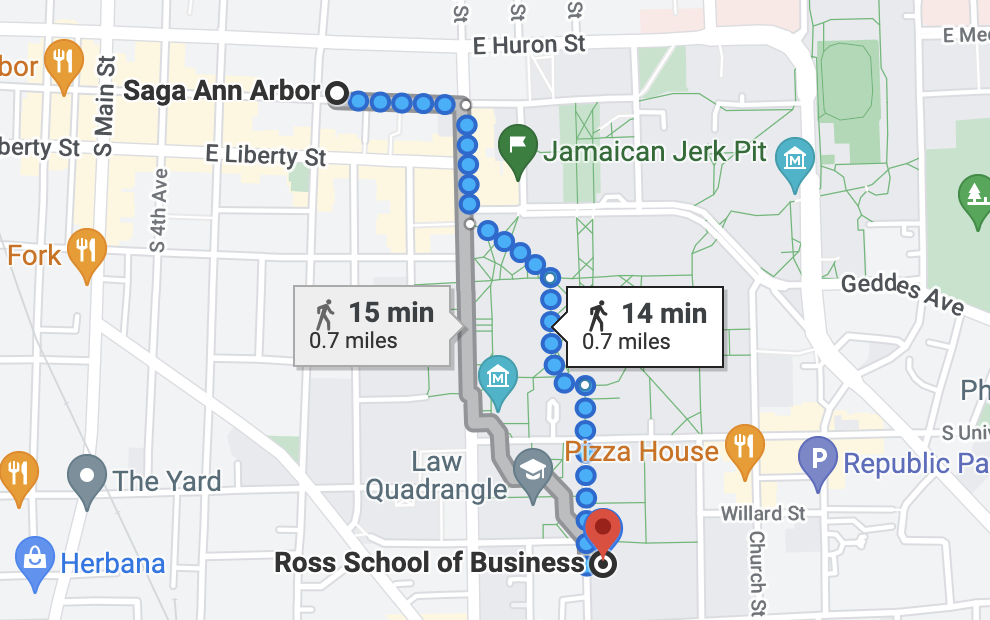
\includegraphics{saga map} \end{center}

\textbf{Website:}
\url{https://www.sagaannarbor.com/}

\textbf{Floor plans:}
1-, 2-, 3-, \& 4-Bedroom Apartments

\textbf{Description:}
Saga Ann Arbor provides students with more than just a place to call home. The off campus housing near University of Michigan is centrally located in Ann Arbor, just minutes from the campus and many local favorites, including restaurants, shopping outlets, and recreation. But residents don't have to go far for fun and relaxation, as our community boasts an array of resort-style amenities that help strike the perfect work-life balance. In addition, the apartments come fully furnished and boast modern interior features. For a UMich living experience unlike any other, look no further than Saga Ann Arbor.

\textbf{Pros:}
Nearby Retail \& Shopping Destinations

\begin{itemize}
\tightlist
\item
  Landmark
\end{itemize}

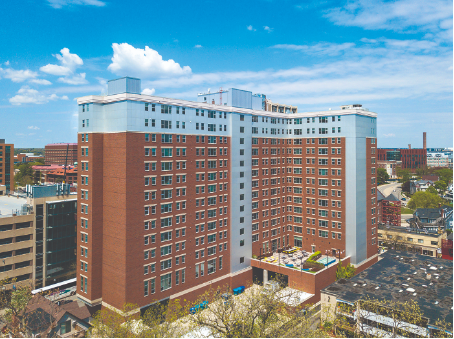
\includegraphics[width=0.32\textwidth,height=\textheight]{landmark_exterior1.png}
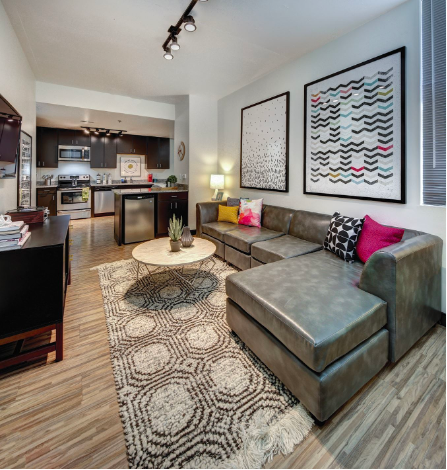
\includegraphics[width=0.3\textwidth,height=\textheight]{landmark_interior.png}
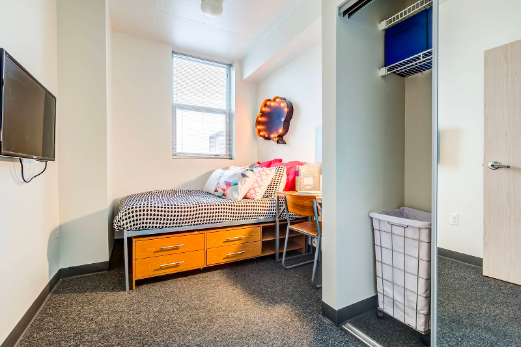
\includegraphics[width=0.35\textwidth,height=\textheight]{landmark_interior2.png}

\begin{center}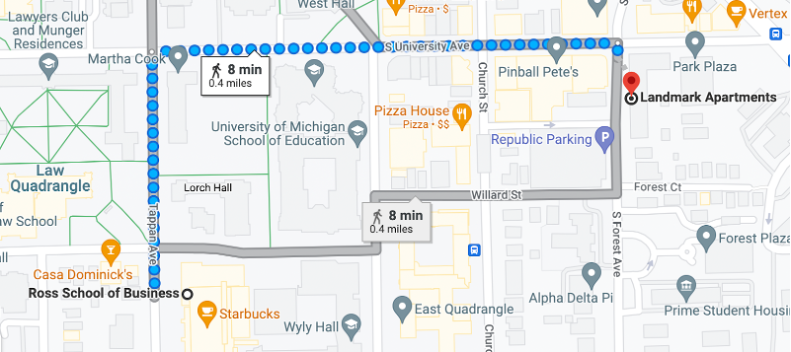
\includegraphics{landmark_map} \end{center}

\textbf{Website:} \url{https://www.livethelandmark.com/}

\textbf{Floor plans:} Studio, 2-, 3-, 4-, 5-, \& 6-Bedroom Apartments

\textbf{Description:} Landmark is a high-rise luxury apartment located just in an 8-minute walk away from Ross. They offer a variety of floor plans from 1 to 6 bedrooms that come with 1 to 4 baths. In terms of pricing, the monthly rent ranges from \$1250 to \$2074.

\textbf{Pros:} Washer and dryer in unit, fully furnished, and amenities include gym, pool, hot tub, study space, garage parking, theater

\begin{itemize}
\tightlist
\item
  z place
\end{itemize}

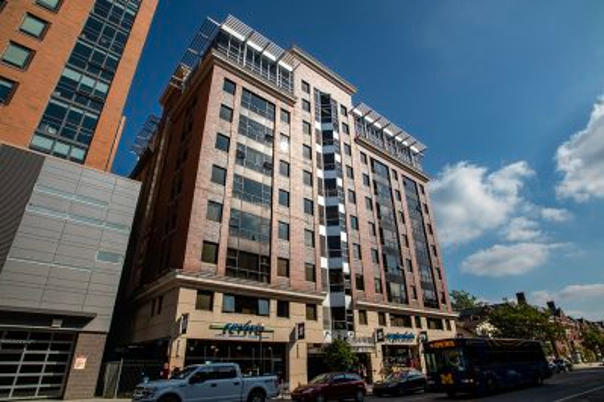
\includegraphics[width=0.36\textwidth,height=\textheight]{zplace_exterior.png}
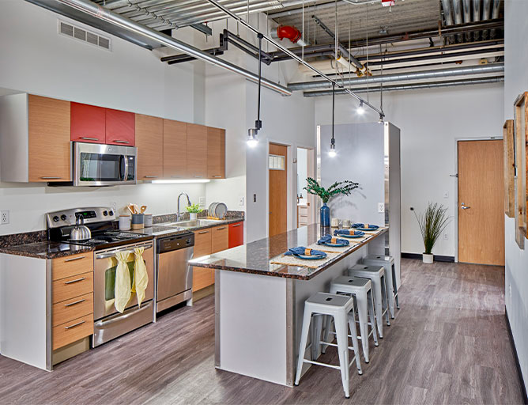
\includegraphics[width=0.32\textwidth,height=\textheight]{zplace_interior1.png}
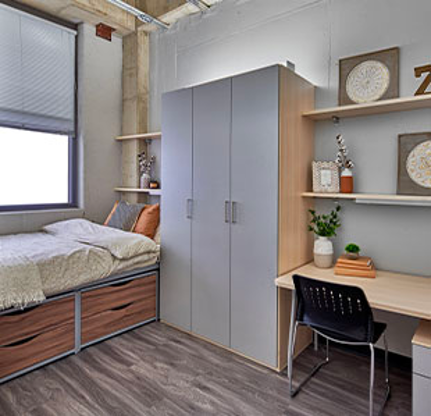
\includegraphics[width=0.3\textwidth,height=\textheight]{zplace_interior2.png}

\begin{center}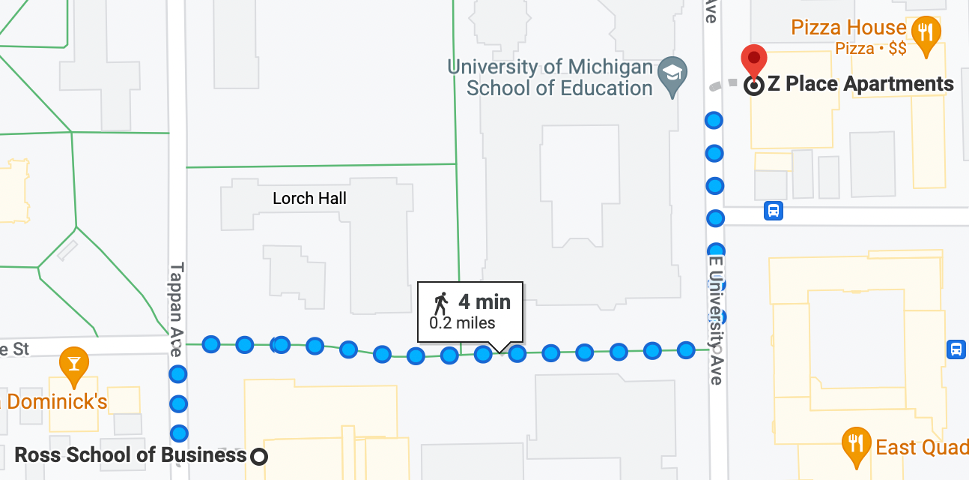
\includegraphics{zplace_map} \end{center}

\textbf{Website:} \url{https://www.zplaceapartments.com/}

\textbf{Floor plans:} 2-, 4-, \& 6-Bedroom Apartments

\textbf{Description:} Located just a 4 minute walk away from the Ross School of Business, Z Place Apartments offers luxury apartment units that will give you feel a sense of home, even when you are away from home.

\textbf{Pros:} Washer and dryer in unit, fully furnished, and amenities include gym, underground parking

\begin{itemize}
\tightlist
\item
  Six11
\end{itemize}

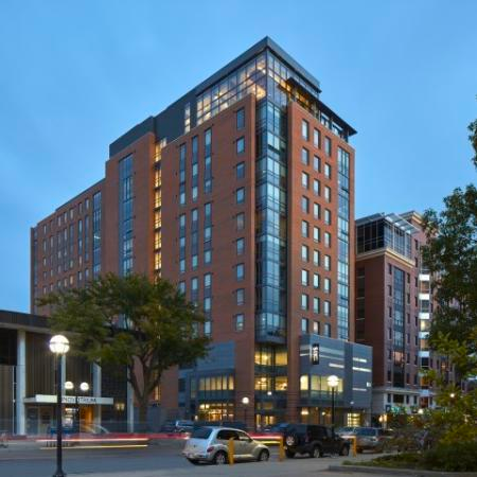
\includegraphics[width=0.33\textwidth,height=\textheight]{611_exterior.png}
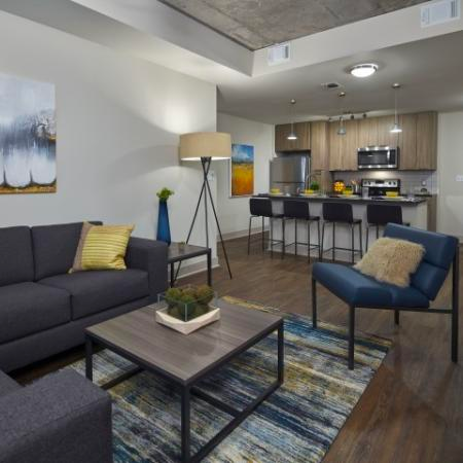
\includegraphics[width=0.32\textwidth,height=\textheight]{611_interior1.png}
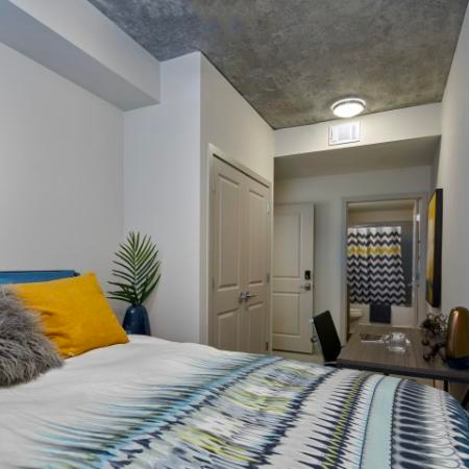
\includegraphics[width=0.33\textwidth,height=\textheight]{611_interior2.png}

\begin{center}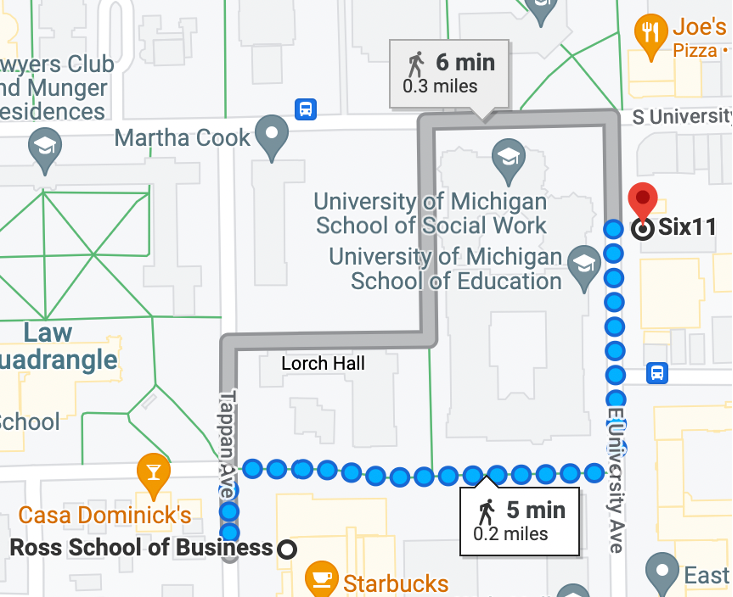
\includegraphics{611_map} \end{center}

\textbf{Website:} \url{https://www.livesix11.com/}

\textbf{Floor plans:} Studio, 4-, 5-, \& 6-Bedroom Apartments

\textbf{Description:} Looking for a luxury apartment just 5 minutes away from Ross? Six11 offers apartment units ranging from \$1489 to \$2359.

\textbf{Pros:} Washer and dryer in unit, fully furnished, and amenities include rooftop terrace, gym, printers, study rooms, parking garage

\hypertarget{south-campus}{%
\subsection{South Campus}\label{south-campus}}

\begin{itemize}
\tightlist
\item
  Hoover and Greene
\end{itemize}

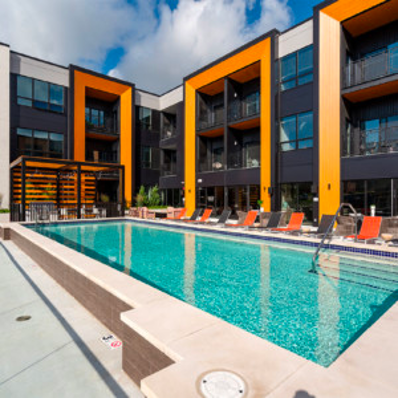
\includegraphics[width=0.32\textwidth,height=\textheight]{HG_exterior.png}
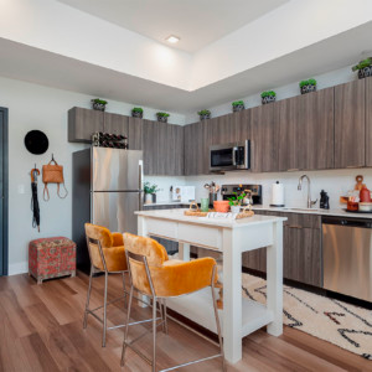
\includegraphics[width=0.32\textwidth,height=\textheight]{HG_interior1.png}
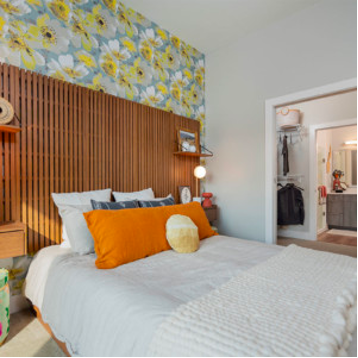
\includegraphics[width=0.32\textwidth,height=\textheight]{HG_interior2.png}

\begin{center}\includegraphics{HG_map} \end{center}

\textbf{Website:} \url{https://hooverandgreene.com/}

\textbf{Floor plans:} Studio, 1-, \& 2-Bedroom Apartments

\textbf{Description:} Hoover and Greene is a luxury apartment complex located on the South side of campus, with close proximity to many of the athletic fields, and most importantly the Big House. Perfect location for any sports fans, as well as anyone studying at Ross.

\textbf{Pros:} Washer and dryer in unit and amenities include gym, working space, courtyard terrace, pool

\begin{itemize}
\tightlist
\item
  618 South Main
\end{itemize}

\includegraphics[width=0.32\textwidth,height=\textheight]{SM_exterior.png}
\includegraphics[width=0.32\textwidth,height=\textheight]{SM_interior1.png}
\includegraphics[width=0.32\textwidth,height=\textheight]{SM_interior2.png}

\begin{center}\includegraphics{SM_map} \end{center}

\textbf{Website:} \url{https://www.618southmain.com/}

\textbf{Floor plans:} Studio, 1-, \& 2-Bedroom Apartments

\textbf{Description:} 618 South Main is another housing option for anyone interested in living on South Campus near the athletic fields. In addition, this is one of the few high-rise, luxury apartments near campus that allows pets.

\textbf{Pros:} Washer and dryer in unit, and amenities include gym, resident lounge, pool and hot tub, and underground parking. 2 pets are allowed but you do have to pay both a one-time fee and monthly rent.

  \bibliography{book.bib,packages.bib}

\end{document}
